\begin{figure}[H] \centering % Created by tikzDevice version 0.12.4 on 2023-07-24 17:06:18
% !TEX encoding = UTF-8 Unicode
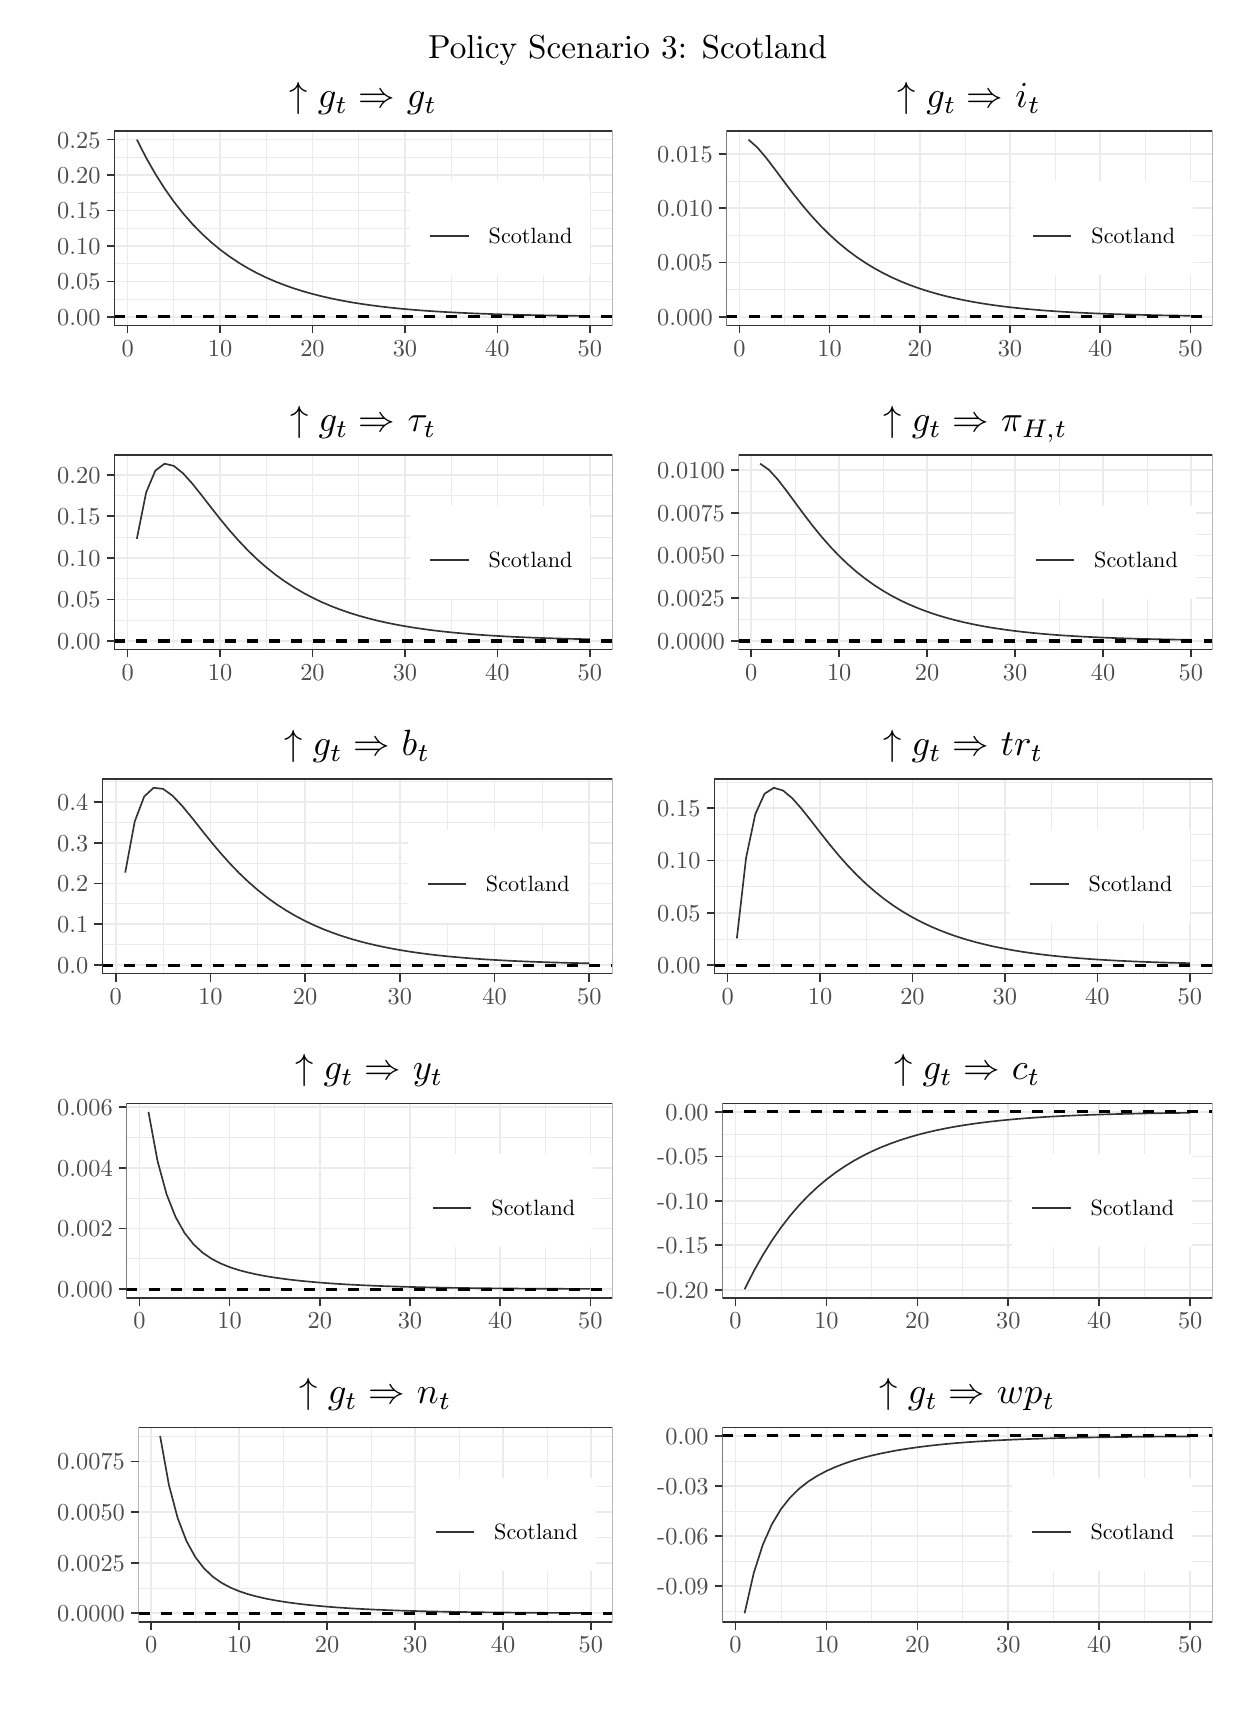
\begin{tikzpicture}[x=1pt,y=1pt]
\definecolor{fillColor}{RGB}{255,255,255}
\path[use as bounding box,fill=fillColor,fill opacity=0.00] (0,0) rectangle (433.62,599.84);
\begin{scope}
\path[clip] (  0.00,468.44) rectangle (216.81,585.55);
\definecolor{drawColor}{RGB}{255,255,255}
\definecolor{fillColor}{RGB}{255,255,255}

\path[draw=drawColor,line width= 0.6pt,line join=round,line cap=round,fill=fillColor] (  0.00,468.44) rectangle (216.81,585.55);
\end{scope}
\begin{scope}
\path[clip] ( 31.27,492.12) rectangle (211.31,562.59);
\definecolor{fillColor}{RGB}{255,255,255}

\path[fill=fillColor] ( 31.27,492.12) rectangle (211.31,562.59);
\definecolor{drawColor}{gray}{0.92}

\path[draw=drawColor,line width= 0.3pt,line join=round] ( 31.27,501.73) --
	(211.31,501.73);

\path[draw=drawColor,line width= 0.3pt,line join=round] ( 31.27,514.54) --
	(211.31,514.54);

\path[draw=drawColor,line width= 0.3pt,line join=round] ( 31.27,527.36) --
	(211.31,527.36);

\path[draw=drawColor,line width= 0.3pt,line join=round] ( 31.27,540.17) --
	(211.31,540.17);

\path[draw=drawColor,line width= 0.3pt,line join=round] ( 31.27,552.98) --
	(211.31,552.98);

\path[draw=drawColor,line width= 0.3pt,line join=round] ( 52.81,492.12) --
	( 52.81,562.59);

\path[draw=drawColor,line width= 0.3pt,line join=round] ( 86.22,492.12) --
	( 86.22,562.59);

\path[draw=drawColor,line width= 0.3pt,line join=round] (119.62,492.12) --
	(119.62,562.59);

\path[draw=drawColor,line width= 0.3pt,line join=round] (153.02,492.12) --
	(153.02,562.59);

\path[draw=drawColor,line width= 0.3pt,line join=round] (186.43,492.12) --
	(186.43,562.59);

\path[draw=drawColor,line width= 0.6pt,line join=round] ( 31.27,495.32) --
	(211.31,495.32);

\path[draw=drawColor,line width= 0.6pt,line join=round] ( 31.27,508.14) --
	(211.31,508.14);

\path[draw=drawColor,line width= 0.6pt,line join=round] ( 31.27,520.95) --
	(211.31,520.95);

\path[draw=drawColor,line width= 0.6pt,line join=round] ( 31.27,533.76) --
	(211.31,533.76);

\path[draw=drawColor,line width= 0.6pt,line join=round] ( 31.27,546.58) --
	(211.31,546.58);

\path[draw=drawColor,line width= 0.6pt,line join=round] ( 31.27,559.39) --
	(211.31,559.39);

\path[draw=drawColor,line width= 0.6pt,line join=round] ( 36.11,492.12) --
	( 36.11,562.59);

\path[draw=drawColor,line width= 0.6pt,line join=round] ( 69.52,492.12) --
	( 69.52,562.59);

\path[draw=drawColor,line width= 0.6pt,line join=round] (102.92,492.12) --
	(102.92,562.59);

\path[draw=drawColor,line width= 0.6pt,line join=round] (136.32,492.12) --
	(136.32,562.59);

\path[draw=drawColor,line width= 0.6pt,line join=round] (169.72,492.12) --
	(169.72,562.59);

\path[draw=drawColor,line width= 0.6pt,line join=round] (203.13,492.12) --
	(203.13,562.59);
\definecolor{drawColor}{gray}{0.20}

\path[draw=drawColor,line width= 0.6pt,line join=round] ( 39.45,559.39) --
	( 42.79,552.85) --
	( 46.13,546.99) --
	( 49.47,541.72) --
	( 52.81,536.98) --
	( 56.15,532.74) --
	( 59.50,528.92) --
	( 62.84,525.49) --
	( 66.18,522.42) --
	( 69.52,519.65) --
	( 72.86,517.17) --
	( 76.20,514.94) --
	( 79.54,512.94) --
	( 82.88,511.14) --
	( 86.22,509.53) --
	( 89.56,508.08) --
	( 92.90,506.78) --
	( 96.24,505.61) --
	( 99.58,504.56) --
	(102.92,503.62) --
	(106.26,502.77) --
	(109.60,502.01) --
	(112.94,501.33) --
	(116.28,500.72) --
	(119.62,500.17) --
	(122.96,499.67) --
	(126.30,499.23) --
	(129.64,498.83) --
	(132.98,498.47) --
	(136.32,498.15) --
	(139.66,497.86) --
	(143.00,497.60) --
	(146.34,497.37) --
	(149.68,497.16) --
	(153.02,496.98) --
	(156.36,496.81) --
	(159.70,496.66) --
	(163.04,496.52) --
	(166.38,496.40) --
	(169.72,496.29) --
	(173.06,496.19) --
	(176.40,496.10) --
	(179.74,496.02) --
	(183.08,495.95) --
	(186.43,495.89) --
	(189.77,495.83) --
	(193.11,495.78) --
	(196.45,495.73) --
	(199.79,495.69) --
	(203.13,495.65);
\definecolor{drawColor}{RGB}{0,0,0}

\path[draw=drawColor,line width= 1.1pt,dash pattern=on 4pt off 4pt ,line join=round] ( 31.27,495.32) -- (211.31,495.32);
\definecolor{drawColor}{gray}{0.20}

\path[draw=drawColor,line width= 0.6pt,line join=round,line cap=round] ( 31.27,492.12) rectangle (211.31,562.59);
\end{scope}
\begin{scope}
\path[clip] (  0.00,  0.00) rectangle (433.62,599.84);
\definecolor{drawColor}{gray}{0.30}

\node[text=drawColor,anchor=base east,inner sep=0pt, outer sep=0pt, scale=  0.88] at ( 26.32,492.29) {0.00};

\node[text=drawColor,anchor=base east,inner sep=0pt, outer sep=0pt, scale=  0.88] at ( 26.32,505.11) {0.05};

\node[text=drawColor,anchor=base east,inner sep=0pt, outer sep=0pt, scale=  0.88] at ( 26.32,517.92) {0.10};

\node[text=drawColor,anchor=base east,inner sep=0pt, outer sep=0pt, scale=  0.88] at ( 26.32,530.73) {0.15};

\node[text=drawColor,anchor=base east,inner sep=0pt, outer sep=0pt, scale=  0.88] at ( 26.32,543.55) {0.20};

\node[text=drawColor,anchor=base east,inner sep=0pt, outer sep=0pt, scale=  0.88] at ( 26.32,556.36) {0.25};
\end{scope}
\begin{scope}
\path[clip] (  0.00,  0.00) rectangle (433.62,599.84);
\definecolor{drawColor}{gray}{0.20}

\path[draw=drawColor,line width= 0.6pt,line join=round] ( 28.52,495.32) --
	( 31.27,495.32);

\path[draw=drawColor,line width= 0.6pt,line join=round] ( 28.52,508.14) --
	( 31.27,508.14);

\path[draw=drawColor,line width= 0.6pt,line join=round] ( 28.52,520.95) --
	( 31.27,520.95);

\path[draw=drawColor,line width= 0.6pt,line join=round] ( 28.52,533.76) --
	( 31.27,533.76);

\path[draw=drawColor,line width= 0.6pt,line join=round] ( 28.52,546.58) --
	( 31.27,546.58);

\path[draw=drawColor,line width= 0.6pt,line join=round] ( 28.52,559.39) --
	( 31.27,559.39);
\end{scope}
\begin{scope}
\path[clip] (  0.00,  0.00) rectangle (433.62,599.84);
\definecolor{drawColor}{gray}{0.20}

\path[draw=drawColor,line width= 0.6pt,line join=round] ( 36.11,489.37) --
	( 36.11,492.12);

\path[draw=drawColor,line width= 0.6pt,line join=round] ( 69.52,489.37) --
	( 69.52,492.12);

\path[draw=drawColor,line width= 0.6pt,line join=round] (102.92,489.37) --
	(102.92,492.12);

\path[draw=drawColor,line width= 0.6pt,line join=round] (136.32,489.37) --
	(136.32,492.12);

\path[draw=drawColor,line width= 0.6pt,line join=round] (169.72,489.37) --
	(169.72,492.12);

\path[draw=drawColor,line width= 0.6pt,line join=round] (203.13,489.37) --
	(203.13,492.12);
\end{scope}
\begin{scope}
\path[clip] (  0.00,  0.00) rectangle (433.62,599.84);
\definecolor{drawColor}{gray}{0.30}

\node[text=drawColor,anchor=base,inner sep=0pt, outer sep=0pt, scale=  0.88] at ( 36.11,481.11) {0};

\node[text=drawColor,anchor=base,inner sep=0pt, outer sep=0pt, scale=  0.88] at ( 69.52,481.11) {10};

\node[text=drawColor,anchor=base,inner sep=0pt, outer sep=0pt, scale=  0.88] at (102.92,481.11) {20};

\node[text=drawColor,anchor=base,inner sep=0pt, outer sep=0pt, scale=  0.88] at (136.32,481.11) {30};

\node[text=drawColor,anchor=base,inner sep=0pt, outer sep=0pt, scale=  0.88] at (169.72,481.11) {40};

\node[text=drawColor,anchor=base,inner sep=0pt, outer sep=0pt, scale=  0.88] at (203.13,481.11) {50};
\end{scope}
\begin{scope}
\path[clip] (  0.00,  0.00) rectangle (433.62,599.84);
\definecolor{fillColor}{RGB}{255,255,255}

\path[fill=fillColor] (138.26,510.43) rectangle (203.35,544.28);
\end{scope}
\begin{scope}
\path[clip] (  0.00,  0.00) rectangle (433.62,599.84);
\definecolor{fillColor}{RGB}{255,255,255}

\path[fill=fillColor] (143.76,515.93) rectangle (161.10,533.28);
\end{scope}
\begin{scope}
\path[clip] (  0.00,  0.00) rectangle (433.62,599.84);
\definecolor{drawColor}{gray}{0.20}

\path[draw=drawColor,line width= 0.6pt,line join=round] (145.49,524.61) -- (159.37,524.61);
\end{scope}
\begin{scope}
\path[clip] (  0.00,  0.00) rectangle (433.62,599.84);
\definecolor{drawColor}{RGB}{0,0,0}

\node[text=drawColor,anchor=base west,inner sep=0pt, outer sep=0pt, scale=  0.80] at (166.60,521.85) {Scotland};
\end{scope}
\begin{scope}
\path[clip] (  0.00,  0.00) rectangle (433.62,599.84);
\definecolor{drawColor}{RGB}{0,0,0}

\node[text=drawColor,anchor=base,inner sep=0pt, outer sep=0pt, scale=  1.32] at (121.29,570.96) {$\uparrow  g_t \Rightarrow $ ${g_t}$};
\end{scope}
\begin{scope}
\path[clip] (216.81,468.44) rectangle (433.62,585.55);
\definecolor{drawColor}{RGB}{255,255,255}
\definecolor{fillColor}{RGB}{255,255,255}

\path[draw=drawColor,line width= 0.6pt,line join=round,line cap=round,fill=fillColor] (216.81,468.44) rectangle (433.62,585.55);
\end{scope}
\begin{scope}
\path[clip] (252.48,492.12) rectangle (428.12,562.59);
\definecolor{fillColor}{RGB}{255,255,255}

\path[fill=fillColor] (252.48,492.12) rectangle (428.12,562.59);
\definecolor{drawColor}{gray}{0.92}

\path[draw=drawColor,line width= 0.3pt,line join=round] (252.48,505.15) --
	(428.12,505.15);

\path[draw=drawColor,line width= 0.3pt,line join=round] (252.48,524.80) --
	(428.12,524.80);

\path[draw=drawColor,line width= 0.3pt,line join=round] (252.48,544.45) --
	(428.12,544.45);

\path[draw=drawColor,line width= 0.3pt,line join=round] (273.50,492.12) --
	(273.50,562.59);

\path[draw=drawColor,line width= 0.3pt,line join=round] (306.08,492.12) --
	(306.08,562.59);

\path[draw=drawColor,line width= 0.3pt,line join=round] (338.67,492.12) --
	(338.67,562.59);

\path[draw=drawColor,line width= 0.3pt,line join=round] (371.26,492.12) --
	(371.26,562.59);

\path[draw=drawColor,line width= 0.3pt,line join=round] (403.84,492.12) --
	(403.84,562.59);

\path[draw=drawColor,line width= 0.6pt,line join=round] (252.48,495.32) --
	(428.12,495.32);

\path[draw=drawColor,line width= 0.6pt,line join=round] (252.48,514.97) --
	(428.12,514.97);

\path[draw=drawColor,line width= 0.6pt,line join=round] (252.48,534.62) --
	(428.12,534.62);

\path[draw=drawColor,line width= 0.6pt,line join=round] (252.48,554.28) --
	(428.12,554.28);

\path[draw=drawColor,line width= 0.6pt,line join=round] (257.20,492.12) --
	(257.20,562.59);

\path[draw=drawColor,line width= 0.6pt,line join=round] (289.79,492.12) --
	(289.79,562.59);

\path[draw=drawColor,line width= 0.6pt,line join=round] (322.38,492.12) --
	(322.38,562.59);

\path[draw=drawColor,line width= 0.6pt,line join=round] (354.96,492.12) --
	(354.96,562.59);

\path[draw=drawColor,line width= 0.6pt,line join=round] (387.55,492.12) --
	(387.55,562.59);

\path[draw=drawColor,line width= 0.6pt,line join=round] (420.14,492.12) --
	(420.14,562.59);
\definecolor{drawColor}{gray}{0.20}

\path[draw=drawColor,line width= 0.6pt,line join=round] (260.46,559.39) --
	(263.72,556.49) --
	(266.98,552.64) --
	(270.24,548.35) --
	(273.50,543.96) --
	(276.76,539.67) --
	(280.01,535.58) --
	(283.27,531.76) --
	(286.53,528.23) --
	(289.79,525.00) --
	(293.05,522.05) --
	(296.31,519.38) --
	(299.57,516.96) --
	(302.82,514.78) --
	(306.08,512.81) --
	(309.34,511.03) --
	(312.60,509.44) --
	(315.86,508.00) --
	(319.12,506.71) --
	(322.38,505.55) --
	(325.64,504.51) --
	(328.89,503.57) --
	(332.15,502.73) --
	(335.41,501.98) --
	(338.67,501.30) --
	(341.93,500.69) --
	(345.19,500.14) --
	(348.45,499.65) --
	(351.70,499.21) --
	(354.96,498.81) --
	(358.22,498.46) --
	(361.48,498.14) --
	(364.74,497.85) --
	(368.00,497.59) --
	(371.26,497.36) --
	(374.52,497.15) --
	(377.77,496.97) --
	(381.03,496.80) --
	(384.29,496.65) --
	(387.55,496.51) --
	(390.81,496.39) --
	(394.07,496.28) --
	(397.33,496.19) --
	(400.58,496.10) --
	(403.84,496.02) --
	(407.10,495.95) --
	(410.36,495.88) --
	(413.62,495.83) --
	(416.88,495.78) --
	(420.14,495.73);
\definecolor{drawColor}{RGB}{0,0,0}

\path[draw=drawColor,line width= 1.1pt,dash pattern=on 4pt off 4pt ,line join=round] (252.48,495.32) -- (428.12,495.32);
\definecolor{drawColor}{gray}{0.20}

\path[draw=drawColor,line width= 0.6pt,line join=round,line cap=round] (252.48,492.12) rectangle (428.12,562.59);
\end{scope}
\begin{scope}
\path[clip] (  0.00,  0.00) rectangle (433.62,599.84);
\definecolor{drawColor}{gray}{0.30}

\node[text=drawColor,anchor=base east,inner sep=0pt, outer sep=0pt, scale=  0.88] at (247.53,492.29) {0.000};

\node[text=drawColor,anchor=base east,inner sep=0pt, outer sep=0pt, scale=  0.88] at (247.53,511.94) {0.005};

\node[text=drawColor,anchor=base east,inner sep=0pt, outer sep=0pt, scale=  0.88] at (247.53,531.59) {0.010};

\node[text=drawColor,anchor=base east,inner sep=0pt, outer sep=0pt, scale=  0.88] at (247.53,551.25) {0.015};
\end{scope}
\begin{scope}
\path[clip] (  0.00,  0.00) rectangle (433.62,599.84);
\definecolor{drawColor}{gray}{0.20}

\path[draw=drawColor,line width= 0.6pt,line join=round] (249.73,495.32) --
	(252.48,495.32);

\path[draw=drawColor,line width= 0.6pt,line join=round] (249.73,514.97) --
	(252.48,514.97);

\path[draw=drawColor,line width= 0.6pt,line join=round] (249.73,534.62) --
	(252.48,534.62);

\path[draw=drawColor,line width= 0.6pt,line join=round] (249.73,554.28) --
	(252.48,554.28);
\end{scope}
\begin{scope}
\path[clip] (  0.00,  0.00) rectangle (433.62,599.84);
\definecolor{drawColor}{gray}{0.20}

\path[draw=drawColor,line width= 0.6pt,line join=round] (257.20,489.37) --
	(257.20,492.12);

\path[draw=drawColor,line width= 0.6pt,line join=round] (289.79,489.37) --
	(289.79,492.12);

\path[draw=drawColor,line width= 0.6pt,line join=round] (322.38,489.37) --
	(322.38,492.12);

\path[draw=drawColor,line width= 0.6pt,line join=round] (354.96,489.37) --
	(354.96,492.12);

\path[draw=drawColor,line width= 0.6pt,line join=round] (387.55,489.37) --
	(387.55,492.12);

\path[draw=drawColor,line width= 0.6pt,line join=round] (420.14,489.37) --
	(420.14,492.12);
\end{scope}
\begin{scope}
\path[clip] (  0.00,  0.00) rectangle (433.62,599.84);
\definecolor{drawColor}{gray}{0.30}

\node[text=drawColor,anchor=base,inner sep=0pt, outer sep=0pt, scale=  0.88] at (257.20,481.11) {0};

\node[text=drawColor,anchor=base,inner sep=0pt, outer sep=0pt, scale=  0.88] at (289.79,481.11) {10};

\node[text=drawColor,anchor=base,inner sep=0pt, outer sep=0pt, scale=  0.88] at (322.38,481.11) {20};

\node[text=drawColor,anchor=base,inner sep=0pt, outer sep=0pt, scale=  0.88] at (354.96,481.11) {30};

\node[text=drawColor,anchor=base,inner sep=0pt, outer sep=0pt, scale=  0.88] at (387.55,481.11) {40};

\node[text=drawColor,anchor=base,inner sep=0pt, outer sep=0pt, scale=  0.88] at (420.14,481.11) {50};
\end{scope}
\begin{scope}
\path[clip] (  0.00,  0.00) rectangle (433.62,599.84);
\definecolor{fillColor}{RGB}{255,255,255}

\path[fill=fillColor] (356.06,510.43) rectangle (421.15,544.28);
\end{scope}
\begin{scope}
\path[clip] (  0.00,  0.00) rectangle (433.62,599.84);
\definecolor{fillColor}{RGB}{255,255,255}

\path[fill=fillColor] (361.56,515.93) rectangle (378.90,533.28);
\end{scope}
\begin{scope}
\path[clip] (  0.00,  0.00) rectangle (433.62,599.84);
\definecolor{drawColor}{gray}{0.20}

\path[draw=drawColor,line width= 0.6pt,line join=round] (363.29,524.61) -- (377.17,524.61);
\end{scope}
\begin{scope}
\path[clip] (  0.00,  0.00) rectangle (433.62,599.84);
\definecolor{drawColor}{RGB}{0,0,0}

\node[text=drawColor,anchor=base west,inner sep=0pt, outer sep=0pt, scale=  0.80] at (384.40,521.85) {Scotland};
\end{scope}
\begin{scope}
\path[clip] (  0.00,  0.00) rectangle (433.62,599.84);
\definecolor{drawColor}{RGB}{0,0,0}

\node[text=drawColor,anchor=base,inner sep=0pt, outer sep=0pt, scale=  1.32] at (340.30,570.96) {$\uparrow  g_t \Rightarrow $ ${i_t}$};
\end{scope}
\begin{scope}
\path[clip] (  0.00,351.33) rectangle (216.81,468.44);
\definecolor{drawColor}{RGB}{255,255,255}
\definecolor{fillColor}{RGB}{255,255,255}

\path[draw=drawColor,line width= 0.6pt,line join=round,line cap=round,fill=fillColor] (  0.00,351.33) rectangle (216.81,468.44);
\end{scope}
\begin{scope}
\path[clip] ( 31.27,375.01) rectangle (211.31,445.48);
\definecolor{fillColor}{RGB}{255,255,255}

\path[fill=fillColor] ( 31.27,375.01) rectangle (211.31,445.48);
\definecolor{drawColor}{gray}{0.92}

\path[draw=drawColor,line width= 0.3pt,line join=round] ( 31.27,385.72) --
	(211.31,385.72);

\path[draw=drawColor,line width= 0.3pt,line join=round] ( 31.27,400.75) --
	(211.31,400.75);

\path[draw=drawColor,line width= 0.3pt,line join=round] ( 31.27,415.77) --
	(211.31,415.77);

\path[draw=drawColor,line width= 0.3pt,line join=round] ( 31.27,430.79) --
	(211.31,430.79);

\path[draw=drawColor,line width= 0.3pt,line join=round] ( 52.81,375.01) --
	( 52.81,445.48);

\path[draw=drawColor,line width= 0.3pt,line join=round] ( 86.22,375.01) --
	( 86.22,445.48);

\path[draw=drawColor,line width= 0.3pt,line join=round] (119.62,375.01) --
	(119.62,445.48);

\path[draw=drawColor,line width= 0.3pt,line join=round] (153.02,375.01) --
	(153.02,445.48);

\path[draw=drawColor,line width= 0.3pt,line join=round] (186.43,375.01) --
	(186.43,445.48);

\path[draw=drawColor,line width= 0.6pt,line join=round] ( 31.27,378.21) --
	(211.31,378.21);

\path[draw=drawColor,line width= 0.6pt,line join=round] ( 31.27,393.24) --
	(211.31,393.24);

\path[draw=drawColor,line width= 0.6pt,line join=round] ( 31.27,408.26) --
	(211.31,408.26);

\path[draw=drawColor,line width= 0.6pt,line join=round] ( 31.27,423.28) --
	(211.31,423.28);

\path[draw=drawColor,line width= 0.6pt,line join=round] ( 31.27,438.30) --
	(211.31,438.30);

\path[draw=drawColor,line width= 0.6pt,line join=round] ( 36.11,375.01) --
	( 36.11,445.48);

\path[draw=drawColor,line width= 0.6pt,line join=round] ( 69.52,375.01) --
	( 69.52,445.48);

\path[draw=drawColor,line width= 0.6pt,line join=round] (102.92,375.01) --
	(102.92,445.48);

\path[draw=drawColor,line width= 0.6pt,line join=round] (136.32,375.01) --
	(136.32,445.48);

\path[draw=drawColor,line width= 0.6pt,line join=round] (169.72,375.01) --
	(169.72,445.48);

\path[draw=drawColor,line width= 0.6pt,line join=round] (203.13,375.01) --
	(203.13,445.48);
\definecolor{drawColor}{gray}{0.20}

\path[draw=drawColor,line width= 0.6pt,line join=round] ( 39.45,415.13) --
	( 42.79,431.85) --
	( 46.13,439.78) --
	( 49.47,442.28) --
	( 52.81,441.49) --
	( 56.15,438.79) --
	( 59.50,435.07) --
	( 62.84,430.88) --
	( 66.18,426.57) --
	( 69.52,422.33) --
	( 72.86,418.28) --
	( 76.20,414.49) --
	( 79.54,410.98) --
	( 82.88,407.76) --
	( 86.22,404.83) --
	( 89.56,402.17) --
	( 92.90,399.76) --
	( 96.24,397.59) --
	( 99.58,395.63) --
	(102.92,393.86) --
	(106.26,392.27) --
	(109.60,390.84) --
	(112.94,389.56) --
	(116.28,388.40) --
	(119.62,387.36) --
	(122.96,386.43) --
	(126.30,385.59) --
	(129.64,384.84) --
	(132.98,384.16) --
	(136.32,383.56) --
	(139.66,383.01) --
	(143.00,382.52) --
	(146.34,382.08) --
	(149.68,381.69) --
	(153.02,381.33) --
	(156.36,381.02) --
	(159.70,380.73) --
	(163.04,380.47) --
	(166.38,380.24) --
	(169.72,380.04) --
	(173.06,379.85) --
	(176.40,379.68) --
	(179.74,379.53) --
	(183.08,379.40) --
	(186.43,379.28) --
	(189.77,379.17) --
	(193.11,379.07) --
	(196.45,378.98) --
	(199.79,378.91) --
	(203.13,378.83);
\definecolor{drawColor}{RGB}{0,0,0}

\path[draw=drawColor,line width= 1.1pt,dash pattern=on 4pt off 4pt ,line join=round] ( 31.27,378.21) -- (211.31,378.21);
\definecolor{drawColor}{gray}{0.20}

\path[draw=drawColor,line width= 0.6pt,line join=round,line cap=round] ( 31.27,375.01) rectangle (211.31,445.48);
\end{scope}
\begin{scope}
\path[clip] (  0.00,  0.00) rectangle (433.62,599.84);
\definecolor{drawColor}{gray}{0.30}

\node[text=drawColor,anchor=base east,inner sep=0pt, outer sep=0pt, scale=  0.88] at ( 26.32,375.18) {0.00};

\node[text=drawColor,anchor=base east,inner sep=0pt, outer sep=0pt, scale=  0.88] at ( 26.32,390.21) {0.05};

\node[text=drawColor,anchor=base east,inner sep=0pt, outer sep=0pt, scale=  0.88] at ( 26.32,405.23) {0.10};

\node[text=drawColor,anchor=base east,inner sep=0pt, outer sep=0pt, scale=  0.88] at ( 26.32,420.25) {0.15};

\node[text=drawColor,anchor=base east,inner sep=0pt, outer sep=0pt, scale=  0.88] at ( 26.32,435.27) {0.20};
\end{scope}
\begin{scope}
\path[clip] (  0.00,  0.00) rectangle (433.62,599.84);
\definecolor{drawColor}{gray}{0.20}

\path[draw=drawColor,line width= 0.6pt,line join=round] ( 28.52,378.21) --
	( 31.27,378.21);

\path[draw=drawColor,line width= 0.6pt,line join=round] ( 28.52,393.24) --
	( 31.27,393.24);

\path[draw=drawColor,line width= 0.6pt,line join=round] ( 28.52,408.26) --
	( 31.27,408.26);

\path[draw=drawColor,line width= 0.6pt,line join=round] ( 28.52,423.28) --
	( 31.27,423.28);

\path[draw=drawColor,line width= 0.6pt,line join=round] ( 28.52,438.30) --
	( 31.27,438.30);
\end{scope}
\begin{scope}
\path[clip] (  0.00,  0.00) rectangle (433.62,599.84);
\definecolor{drawColor}{gray}{0.20}

\path[draw=drawColor,line width= 0.6pt,line join=round] ( 36.11,372.26) --
	( 36.11,375.01);

\path[draw=drawColor,line width= 0.6pt,line join=round] ( 69.52,372.26) --
	( 69.52,375.01);

\path[draw=drawColor,line width= 0.6pt,line join=round] (102.92,372.26) --
	(102.92,375.01);

\path[draw=drawColor,line width= 0.6pt,line join=round] (136.32,372.26) --
	(136.32,375.01);

\path[draw=drawColor,line width= 0.6pt,line join=round] (169.72,372.26) --
	(169.72,375.01);

\path[draw=drawColor,line width= 0.6pt,line join=round] (203.13,372.26) --
	(203.13,375.01);
\end{scope}
\begin{scope}
\path[clip] (  0.00,  0.00) rectangle (433.62,599.84);
\definecolor{drawColor}{gray}{0.30}

\node[text=drawColor,anchor=base,inner sep=0pt, outer sep=0pt, scale=  0.88] at ( 36.11,364.00) {0};

\node[text=drawColor,anchor=base,inner sep=0pt, outer sep=0pt, scale=  0.88] at ( 69.52,364.00) {10};

\node[text=drawColor,anchor=base,inner sep=0pt, outer sep=0pt, scale=  0.88] at (102.92,364.00) {20};

\node[text=drawColor,anchor=base,inner sep=0pt, outer sep=0pt, scale=  0.88] at (136.32,364.00) {30};

\node[text=drawColor,anchor=base,inner sep=0pt, outer sep=0pt, scale=  0.88] at (169.72,364.00) {40};

\node[text=drawColor,anchor=base,inner sep=0pt, outer sep=0pt, scale=  0.88] at (203.13,364.00) {50};
\end{scope}
\begin{scope}
\path[clip] (  0.00,  0.00) rectangle (433.62,599.84);
\definecolor{fillColor}{RGB}{255,255,255}

\path[fill=fillColor] (138.26,393.32) rectangle (203.35,427.17);
\end{scope}
\begin{scope}
\path[clip] (  0.00,  0.00) rectangle (433.62,599.84);
\definecolor{fillColor}{RGB}{255,255,255}

\path[fill=fillColor] (143.76,398.82) rectangle (161.10,416.17);
\end{scope}
\begin{scope}
\path[clip] (  0.00,  0.00) rectangle (433.62,599.84);
\definecolor{drawColor}{gray}{0.20}

\path[draw=drawColor,line width= 0.6pt,line join=round] (145.49,407.50) -- (159.37,407.50);
\end{scope}
\begin{scope}
\path[clip] (  0.00,  0.00) rectangle (433.62,599.84);
\definecolor{drawColor}{RGB}{0,0,0}

\node[text=drawColor,anchor=base west,inner sep=0pt, outer sep=0pt, scale=  0.80] at (166.60,404.74) {Scotland};
\end{scope}
\begin{scope}
\path[clip] (  0.00,  0.00) rectangle (433.62,599.84);
\definecolor{drawColor}{RGB}{0,0,0}

\node[text=drawColor,anchor=base,inner sep=0pt, outer sep=0pt, scale=  1.32] at (121.29,453.85) {$\uparrow  g_t \Rightarrow $ ${\tau_t}$};
\end{scope}
\begin{scope}
\path[clip] (216.81,351.33) rectangle (433.62,468.44);
\definecolor{drawColor}{RGB}{255,255,255}
\definecolor{fillColor}{RGB}{255,255,255}

\path[draw=drawColor,line width= 0.6pt,line join=round,line cap=round,fill=fillColor] (216.81,351.33) rectangle (433.62,468.44);
\end{scope}
\begin{scope}
\path[clip] (256.88,375.01) rectangle (428.12,445.48);
\definecolor{fillColor}{RGB}{255,255,255}

\path[fill=fillColor] (256.88,375.01) rectangle (428.12,445.48);
\definecolor{drawColor}{gray}{0.92}

\path[draw=drawColor,line width= 0.3pt,line join=round] (256.88,385.93) --
	(428.12,385.93);

\path[draw=drawColor,line width= 0.3pt,line join=round] (256.88,401.36) --
	(428.12,401.36);

\path[draw=drawColor,line width= 0.3pt,line join=round] (256.88,416.79) --
	(428.12,416.79);

\path[draw=drawColor,line width= 0.3pt,line join=round] (256.88,432.22) --
	(428.12,432.22);

\path[draw=drawColor,line width= 0.3pt,line join=round] (277.37,375.01) --
	(277.37,445.48);

\path[draw=drawColor,line width= 0.3pt,line join=round] (309.14,375.01) --
	(309.14,445.48);

\path[draw=drawColor,line width= 0.3pt,line join=round] (340.91,375.01) --
	(340.91,445.48);

\path[draw=drawColor,line width= 0.3pt,line join=round] (372.68,375.01) --
	(372.68,445.48);

\path[draw=drawColor,line width= 0.3pt,line join=round] (404.45,375.01) --
	(404.45,445.48);

\path[draw=drawColor,line width= 0.6pt,line join=round] (256.88,378.21) --
	(428.12,378.21);

\path[draw=drawColor,line width= 0.6pt,line join=round] (256.88,393.64) --
	(428.12,393.64);

\path[draw=drawColor,line width= 0.6pt,line join=round] (256.88,409.07) --
	(428.12,409.07);

\path[draw=drawColor,line width= 0.6pt,line join=round] (256.88,424.50) --
	(428.12,424.50);

\path[draw=drawColor,line width= 0.6pt,line join=round] (256.88,439.93) --
	(428.12,439.93);

\path[draw=drawColor,line width= 0.6pt,line join=round] (261.48,375.01) --
	(261.48,445.48);

\path[draw=drawColor,line width= 0.6pt,line join=round] (293.25,375.01) --
	(293.25,445.48);

\path[draw=drawColor,line width= 0.6pt,line join=round] (325.03,375.01) --
	(325.03,445.48);

\path[draw=drawColor,line width= 0.6pt,line join=round] (356.80,375.01) --
	(356.80,445.48);

\path[draw=drawColor,line width= 0.6pt,line join=round] (388.57,375.01) --
	(388.57,445.48);

\path[draw=drawColor,line width= 0.6pt,line join=round] (420.34,375.01) --
	(420.34,445.48);
\definecolor{drawColor}{gray}{0.20}

\path[draw=drawColor,line width= 0.6pt,line join=round] (264.66,442.28) --
	(267.84,440.08) --
	(271.02,436.60) --
	(274.19,432.50) --
	(277.37,428.18) --
	(280.55,423.88) --
	(283.72,419.74) --
	(286.90,415.85) --
	(290.08,412.23) --
	(293.25,408.91) --
	(296.43,405.87) --
	(299.61,403.11) --
	(302.79,400.61) --
	(305.96,398.36) --
	(309.14,396.32) --
	(312.32,394.48) --
	(315.49,392.83) --
	(318.67,391.35) --
	(321.85,390.01) --
	(325.03,388.81) --
	(328.20,387.73) --
	(331.38,386.76) --
	(334.56,385.89) --
	(337.73,385.11) --
	(340.91,384.40) --
	(344.09,383.77) --
	(347.26,383.20) --
	(350.44,382.70) --
	(353.62,382.24) --
	(356.80,381.83) --
	(359.97,381.46) --
	(363.15,381.13) --
	(366.33,380.83) --
	(369.50,380.56) --
	(372.68,380.32) --
	(375.86,380.11) --
	(379.03,379.92) --
	(382.21,379.74) --
	(385.39,379.59) --
	(388.57,379.45) --
	(391.74,379.32) --
	(394.92,379.21) --
	(398.10,379.11) --
	(401.27,379.01) --
	(404.45,378.93) --
	(407.63,378.86) --
	(410.81,378.79) --
	(413.98,378.73) --
	(417.16,378.68) --
	(420.34,378.63);
\definecolor{drawColor}{RGB}{0,0,0}

\path[draw=drawColor,line width= 1.1pt,dash pattern=on 4pt off 4pt ,line join=round] (256.88,378.21) -- (428.12,378.21);
\definecolor{drawColor}{gray}{0.20}

\path[draw=drawColor,line width= 0.6pt,line join=round,line cap=round] (256.88,375.01) rectangle (428.12,445.48);
\end{scope}
\begin{scope}
\path[clip] (  0.00,  0.00) rectangle (433.62,599.84);
\definecolor{drawColor}{gray}{0.30}

\node[text=drawColor,anchor=base east,inner sep=0pt, outer sep=0pt, scale=  0.88] at (251.93,375.18) {0.0000};

\node[text=drawColor,anchor=base east,inner sep=0pt, outer sep=0pt, scale=  0.88] at (251.93,390.61) {0.0025};

\node[text=drawColor,anchor=base east,inner sep=0pt, outer sep=0pt, scale=  0.88] at (251.93,406.04) {0.0050};

\node[text=drawColor,anchor=base east,inner sep=0pt, outer sep=0pt, scale=  0.88] at (251.93,421.47) {0.0075};

\node[text=drawColor,anchor=base east,inner sep=0pt, outer sep=0pt, scale=  0.88] at (251.93,436.90) {0.0100};
\end{scope}
\begin{scope}
\path[clip] (  0.00,  0.00) rectangle (433.62,599.84);
\definecolor{drawColor}{gray}{0.20}

\path[draw=drawColor,line width= 0.6pt,line join=round] (254.13,378.21) --
	(256.88,378.21);

\path[draw=drawColor,line width= 0.6pt,line join=round] (254.13,393.64) --
	(256.88,393.64);

\path[draw=drawColor,line width= 0.6pt,line join=round] (254.13,409.07) --
	(256.88,409.07);

\path[draw=drawColor,line width= 0.6pt,line join=round] (254.13,424.50) --
	(256.88,424.50);

\path[draw=drawColor,line width= 0.6pt,line join=round] (254.13,439.93) --
	(256.88,439.93);
\end{scope}
\begin{scope}
\path[clip] (  0.00,  0.00) rectangle (433.62,599.84);
\definecolor{drawColor}{gray}{0.20}

\path[draw=drawColor,line width= 0.6pt,line join=round] (261.48,372.26) --
	(261.48,375.01);

\path[draw=drawColor,line width= 0.6pt,line join=round] (293.25,372.26) --
	(293.25,375.01);

\path[draw=drawColor,line width= 0.6pt,line join=round] (325.03,372.26) --
	(325.03,375.01);

\path[draw=drawColor,line width= 0.6pt,line join=round] (356.80,372.26) --
	(356.80,375.01);

\path[draw=drawColor,line width= 0.6pt,line join=round] (388.57,372.26) --
	(388.57,375.01);

\path[draw=drawColor,line width= 0.6pt,line join=round] (420.34,372.26) --
	(420.34,375.01);
\end{scope}
\begin{scope}
\path[clip] (  0.00,  0.00) rectangle (433.62,599.84);
\definecolor{drawColor}{gray}{0.30}

\node[text=drawColor,anchor=base,inner sep=0pt, outer sep=0pt, scale=  0.88] at (261.48,364.00) {0};

\node[text=drawColor,anchor=base,inner sep=0pt, outer sep=0pt, scale=  0.88] at (293.25,364.00) {10};

\node[text=drawColor,anchor=base,inner sep=0pt, outer sep=0pt, scale=  0.88] at (325.03,364.00) {20};

\node[text=drawColor,anchor=base,inner sep=0pt, outer sep=0pt, scale=  0.88] at (356.80,364.00) {30};

\node[text=drawColor,anchor=base,inner sep=0pt, outer sep=0pt, scale=  0.88] at (388.57,364.00) {40};

\node[text=drawColor,anchor=base,inner sep=0pt, outer sep=0pt, scale=  0.88] at (420.34,364.00) {50};
\end{scope}
\begin{scope}
\path[clip] (  0.00,  0.00) rectangle (433.62,599.84);
\definecolor{fillColor}{RGB}{255,255,255}

\path[fill=fillColor] (357.05,393.32) rectangle (422.14,427.17);
\end{scope}
\begin{scope}
\path[clip] (  0.00,  0.00) rectangle (433.62,599.84);
\definecolor{fillColor}{RGB}{255,255,255}

\path[fill=fillColor] (362.55,398.82) rectangle (379.89,416.17);
\end{scope}
\begin{scope}
\path[clip] (  0.00,  0.00) rectangle (433.62,599.84);
\definecolor{drawColor}{gray}{0.20}

\path[draw=drawColor,line width= 0.6pt,line join=round] (364.28,407.50) -- (378.16,407.50);
\end{scope}
\begin{scope}
\path[clip] (  0.00,  0.00) rectangle (433.62,599.84);
\definecolor{drawColor}{RGB}{0,0,0}

\node[text=drawColor,anchor=base west,inner sep=0pt, outer sep=0pt, scale=  0.80] at (385.39,404.74) {Scotland};
\end{scope}
\begin{scope}
\path[clip] (  0.00,  0.00) rectangle (433.62,599.84);
\definecolor{drawColor}{RGB}{0,0,0}

\node[text=drawColor,anchor=base,inner sep=0pt, outer sep=0pt, scale=  1.32] at (342.50,453.85) {$\uparrow  g_t \Rightarrow $ ${\pi_{H,t}}$};
\end{scope}
\begin{scope}
\path[clip] (  0.00,234.22) rectangle (216.81,351.33);
\definecolor{drawColor}{RGB}{255,255,255}
\definecolor{fillColor}{RGB}{255,255,255}

\path[draw=drawColor,line width= 0.6pt,line join=round,line cap=round,fill=fillColor] (  0.00,234.22) rectangle (216.81,351.33);
\end{scope}
\begin{scope}
\path[clip] ( 26.87,257.90) rectangle (211.31,328.37);
\definecolor{fillColor}{RGB}{255,255,255}

\path[fill=fillColor] ( 26.87,257.90) rectangle (211.31,328.37);
\definecolor{drawColor}{gray}{0.92}

\path[draw=drawColor,line width= 0.3pt,line join=round] ( 26.87,268.47) --
	(211.31,268.47);

\path[draw=drawColor,line width= 0.3pt,line join=round] ( 26.87,283.21) --
	(211.31,283.21);

\path[draw=drawColor,line width= 0.3pt,line join=round] ( 26.87,297.94) --
	(211.31,297.94);

\path[draw=drawColor,line width= 0.3pt,line join=round] ( 26.87,312.68) --
	(211.31,312.68);

\path[draw=drawColor,line width= 0.3pt,line join=round] ( 26.87,327.42) --
	(211.31,327.42);

\path[draw=drawColor,line width= 0.3pt,line join=round] ( 48.94,257.90) --
	( 48.94,328.37);

\path[draw=drawColor,line width= 0.3pt,line join=round] ( 83.16,257.90) --
	( 83.16,328.37);

\path[draw=drawColor,line width= 0.3pt,line join=round] (117.38,257.90) --
	(117.38,328.37);

\path[draw=drawColor,line width= 0.3pt,line join=round] (151.60,257.90) --
	(151.60,328.37);

\path[draw=drawColor,line width= 0.3pt,line join=round] (185.82,257.90) --
	(185.82,328.37);

\path[draw=drawColor,line width= 0.6pt,line join=round] ( 26.87,261.10) --
	(211.31,261.10);

\path[draw=drawColor,line width= 0.6pt,line join=round] ( 26.87,275.84) --
	(211.31,275.84);

\path[draw=drawColor,line width= 0.6pt,line join=round] ( 26.87,290.57) --
	(211.31,290.57);

\path[draw=drawColor,line width= 0.6pt,line join=round] ( 26.87,305.31) --
	(211.31,305.31);

\path[draw=drawColor,line width= 0.6pt,line join=round] ( 26.87,320.05) --
	(211.31,320.05);

\path[draw=drawColor,line width= 0.6pt,line join=round] ( 31.83,257.90) --
	( 31.83,328.37);

\path[draw=drawColor,line width= 0.6pt,line join=round] ( 66.05,257.90) --
	( 66.05,328.37);

\path[draw=drawColor,line width= 0.6pt,line join=round] (100.27,257.90) --
	(100.27,328.37);

\path[draw=drawColor,line width= 0.6pt,line join=round] (134.49,257.90) --
	(134.49,328.37);

\path[draw=drawColor,line width= 0.6pt,line join=round] (168.71,257.90) --
	(168.71,328.37);

\path[draw=drawColor,line width= 0.6pt,line join=round] (202.93,257.90) --
	(202.93,328.37);
\definecolor{drawColor}{gray}{0.20}

\path[draw=drawColor,line width= 0.6pt,line join=round] ( 35.25,294.52) --
	( 38.68,312.98) --
	( 42.10,322.01) --
	( 45.52,325.17) --
	( 48.94,324.77) --
	( 52.36,322.29) --
	( 55.79,318.67) --
	( 59.21,314.52) --
	( 62.63,310.20) --
	( 66.05,305.93) --
	( 69.47,301.84) --
	( 72.90,298.00) --
	( 76.32,294.44) --
	( 79.74,291.18) --
	( 83.16,288.20) --
	( 86.58,285.49) --
	( 90.00,283.04) --
	( 93.43,280.83) --
	( 96.85,278.83) --
	(100.27,277.04) --
	(103.69,275.42) --
	(107.11,273.96) --
	(110.54,272.65) --
	(113.96,271.48) --
	(117.38,270.42) --
	(120.80,269.47) --
	(124.22,268.62) --
	(127.65,267.85) --
	(131.07,267.16) --
	(134.49,266.54) --
	(137.91,265.99) --
	(141.33,265.49) --
	(144.75,265.04) --
	(148.18,264.64) --
	(151.60,264.28) --
	(155.02,263.96) --
	(158.44,263.67) --
	(161.86,263.40) --
	(165.29,263.17) --
	(168.71,262.96) --
	(172.13,262.77) --
	(175.55,262.60) --
	(178.97,262.45) --
	(182.40,262.31) --
	(185.82,262.19) --
	(189.24,262.08) --
	(192.66,261.98) --
	(196.08,261.89) --
	(199.50,261.81) --
	(202.93,261.74);
\definecolor{drawColor}{RGB}{0,0,0}

\path[draw=drawColor,line width= 1.1pt,dash pattern=on 4pt off 4pt ,line join=round] ( 26.87,261.10) -- (211.31,261.10);
\definecolor{drawColor}{gray}{0.20}

\path[draw=drawColor,line width= 0.6pt,line join=round,line cap=round] ( 26.87,257.90) rectangle (211.31,328.37);
\end{scope}
\begin{scope}
\path[clip] (  0.00,  0.00) rectangle (433.62,599.84);
\definecolor{drawColor}{gray}{0.30}

\node[text=drawColor,anchor=base east,inner sep=0pt, outer sep=0pt, scale=  0.88] at ( 21.92,258.07) {0.0};

\node[text=drawColor,anchor=base east,inner sep=0pt, outer sep=0pt, scale=  0.88] at ( 21.92,272.81) {0.1};

\node[text=drawColor,anchor=base east,inner sep=0pt, outer sep=0pt, scale=  0.88] at ( 21.92,287.54) {0.2};

\node[text=drawColor,anchor=base east,inner sep=0pt, outer sep=0pt, scale=  0.88] at ( 21.92,302.28) {0.3};

\node[text=drawColor,anchor=base east,inner sep=0pt, outer sep=0pt, scale=  0.88] at ( 21.92,317.02) {0.4};
\end{scope}
\begin{scope}
\path[clip] (  0.00,  0.00) rectangle (433.62,599.84);
\definecolor{drawColor}{gray}{0.20}

\path[draw=drawColor,line width= 0.6pt,line join=round] ( 24.12,261.10) --
	( 26.87,261.10);

\path[draw=drawColor,line width= 0.6pt,line join=round] ( 24.12,275.84) --
	( 26.87,275.84);

\path[draw=drawColor,line width= 0.6pt,line join=round] ( 24.12,290.57) --
	( 26.87,290.57);

\path[draw=drawColor,line width= 0.6pt,line join=round] ( 24.12,305.31) --
	( 26.87,305.31);

\path[draw=drawColor,line width= 0.6pt,line join=round] ( 24.12,320.05) --
	( 26.87,320.05);
\end{scope}
\begin{scope}
\path[clip] (  0.00,  0.00) rectangle (433.62,599.84);
\definecolor{drawColor}{gray}{0.20}

\path[draw=drawColor,line width= 0.6pt,line join=round] ( 31.83,255.15) --
	( 31.83,257.90);

\path[draw=drawColor,line width= 0.6pt,line join=round] ( 66.05,255.15) --
	( 66.05,257.90);

\path[draw=drawColor,line width= 0.6pt,line join=round] (100.27,255.15) --
	(100.27,257.90);

\path[draw=drawColor,line width= 0.6pt,line join=round] (134.49,255.15) --
	(134.49,257.90);

\path[draw=drawColor,line width= 0.6pt,line join=round] (168.71,255.15) --
	(168.71,257.90);

\path[draw=drawColor,line width= 0.6pt,line join=round] (202.93,255.15) --
	(202.93,257.90);
\end{scope}
\begin{scope}
\path[clip] (  0.00,  0.00) rectangle (433.62,599.84);
\definecolor{drawColor}{gray}{0.30}

\node[text=drawColor,anchor=base,inner sep=0pt, outer sep=0pt, scale=  0.88] at ( 31.83,246.89) {0};

\node[text=drawColor,anchor=base,inner sep=0pt, outer sep=0pt, scale=  0.88] at ( 66.05,246.89) {10};

\node[text=drawColor,anchor=base,inner sep=0pt, outer sep=0pt, scale=  0.88] at (100.27,246.89) {20};

\node[text=drawColor,anchor=base,inner sep=0pt, outer sep=0pt, scale=  0.88] at (134.49,246.89) {30};

\node[text=drawColor,anchor=base,inner sep=0pt, outer sep=0pt, scale=  0.88] at (168.71,246.89) {40};

\node[text=drawColor,anchor=base,inner sep=0pt, outer sep=0pt, scale=  0.88] at (202.93,246.89) {50};
\end{scope}
\begin{scope}
\path[clip] (  0.00,  0.00) rectangle (433.62,599.84);
\definecolor{fillColor}{RGB}{255,255,255}

\path[fill=fillColor] (137.27,276.21) rectangle (202.36,310.06);
\end{scope}
\begin{scope}
\path[clip] (  0.00,  0.00) rectangle (433.62,599.84);
\definecolor{fillColor}{RGB}{255,255,255}

\path[fill=fillColor] (142.77,281.71) rectangle (160.11,299.06);
\end{scope}
\begin{scope}
\path[clip] (  0.00,  0.00) rectangle (433.62,599.84);
\definecolor{drawColor}{gray}{0.20}

\path[draw=drawColor,line width= 0.6pt,line join=round] (144.50,290.38) -- (158.38,290.38);
\end{scope}
\begin{scope}
\path[clip] (  0.00,  0.00) rectangle (433.62,599.84);
\definecolor{drawColor}{RGB}{0,0,0}

\node[text=drawColor,anchor=base west,inner sep=0pt, outer sep=0pt, scale=  0.80] at (165.61,287.63) {Scotland};
\end{scope}
\begin{scope}
\path[clip] (  0.00,  0.00) rectangle (433.62,599.84);
\definecolor{drawColor}{RGB}{0,0,0}

\node[text=drawColor,anchor=base,inner sep=0pt, outer sep=0pt, scale=  1.32] at (119.09,336.74) {$\uparrow  g_t \Rightarrow $ ${b_t}$};
\end{scope}
\begin{scope}
\path[clip] (216.81,234.22) rectangle (433.62,351.33);
\definecolor{drawColor}{RGB}{255,255,255}
\definecolor{fillColor}{RGB}{255,255,255}

\path[draw=drawColor,line width= 0.6pt,line join=round,line cap=round,fill=fillColor] (216.81,234.22) rectangle (433.62,351.33);
\end{scope}
\begin{scope}
\path[clip] (248.08,257.90) rectangle (428.12,328.37);
\definecolor{fillColor}{RGB}{255,255,255}

\path[fill=fillColor] (248.08,257.90) rectangle (428.12,328.37);
\definecolor{drawColor}{gray}{0.92}

\path[draw=drawColor,line width= 0.3pt,line join=round] (248.08,270.55) --
	(428.12,270.55);

\path[draw=drawColor,line width= 0.3pt,line join=round] (248.08,289.43) --
	(428.12,289.43);

\path[draw=drawColor,line width= 0.3pt,line join=round] (248.08,308.32) --
	(428.12,308.32);

\path[draw=drawColor,line width= 0.3pt,line join=round] (248.08,327.20) --
	(428.12,327.20);

\path[draw=drawColor,line width= 0.3pt,line join=round] (269.62,257.90) --
	(269.62,328.37);

\path[draw=drawColor,line width= 0.3pt,line join=round] (303.03,257.90) --
	(303.03,328.37);

\path[draw=drawColor,line width= 0.3pt,line join=round] (336.43,257.90) --
	(336.43,328.37);

\path[draw=drawColor,line width= 0.3pt,line join=round] (369.83,257.90) --
	(369.83,328.37);

\path[draw=drawColor,line width= 0.3pt,line join=round] (403.24,257.90) --
	(403.24,328.37);

\path[draw=drawColor,line width= 0.6pt,line join=round] (248.08,261.10) --
	(428.12,261.10);

\path[draw=drawColor,line width= 0.6pt,line join=round] (248.08,279.99) --
	(428.12,279.99);

\path[draw=drawColor,line width= 0.6pt,line join=round] (248.08,298.87) --
	(428.12,298.87);

\path[draw=drawColor,line width= 0.6pt,line join=round] (248.08,317.76) --
	(428.12,317.76);

\path[draw=drawColor,line width= 0.6pt,line join=round] (252.92,257.90) --
	(252.92,328.37);

\path[draw=drawColor,line width= 0.6pt,line join=round] (286.33,257.90) --
	(286.33,328.37);

\path[draw=drawColor,line width= 0.6pt,line join=round] (319.73,257.90) --
	(319.73,328.37);

\path[draw=drawColor,line width= 0.6pt,line join=round] (353.13,257.90) --
	(353.13,328.37);

\path[draw=drawColor,line width= 0.6pt,line join=round] (386.53,257.90) --
	(386.53,328.37);

\path[draw=drawColor,line width= 0.6pt,line join=round] (419.94,257.90) --
	(419.94,328.37);
\definecolor{drawColor}{gray}{0.20}

\path[draw=drawColor,line width= 0.6pt,line join=round] (256.26,270.73) --
	(259.60,299.90) --
	(262.94,315.68) --
	(266.28,323.03) --
	(269.62,325.17) --
	(272.96,324.17) --
	(276.31,321.36) --
	(279.65,317.58) --
	(282.99,313.37) --
	(286.33,309.06) --
	(289.67,304.83) --
	(293.01,300.80) --
	(296.35,297.04) --
	(299.69,293.56) --
	(303.03,290.37) --
	(306.37,287.47) --
	(309.71,284.83) --
	(313.05,282.44) --
	(316.39,280.29) --
	(319.73,278.35) --
	(323.07,276.60) --
	(326.41,275.02) --
	(329.75,273.61) --
	(333.09,272.33) --
	(336.43,271.19) --
	(339.77,270.16) --
	(343.11,269.24) --
	(346.45,268.41) --
	(349.79,267.66) --
	(353.13,267.00) --
	(356.47,266.39) --
	(359.81,265.85) --
	(363.15,265.37) --
	(366.49,264.93) --
	(369.83,264.54) --
	(373.17,264.19) --
	(376.51,263.88) --
	(379.85,263.59) --
	(383.19,263.34) --
	(386.53,263.11) --
	(389.87,262.91) --
	(393.21,262.72) --
	(396.55,262.56) --
	(399.89,262.41) --
	(403.24,262.28) --
	(406.58,262.16) --
	(409.92,262.05) --
	(413.26,261.95) --
	(416.60,261.87) --
	(419.94,261.79);
\definecolor{drawColor}{RGB}{0,0,0}

\path[draw=drawColor,line width= 1.1pt,dash pattern=on 4pt off 4pt ,line join=round] (248.08,261.10) -- (428.12,261.10);
\definecolor{drawColor}{gray}{0.20}

\path[draw=drawColor,line width= 0.6pt,line join=round,line cap=round] (248.08,257.90) rectangle (428.12,328.37);
\end{scope}
\begin{scope}
\path[clip] (  0.00,  0.00) rectangle (433.62,599.84);
\definecolor{drawColor}{gray}{0.30}

\node[text=drawColor,anchor=base east,inner sep=0pt, outer sep=0pt, scale=  0.88] at (243.13,258.07) {0.00};

\node[text=drawColor,anchor=base east,inner sep=0pt, outer sep=0pt, scale=  0.88] at (243.13,276.96) {0.05};

\node[text=drawColor,anchor=base east,inner sep=0pt, outer sep=0pt, scale=  0.88] at (243.13,295.84) {0.10};

\node[text=drawColor,anchor=base east,inner sep=0pt, outer sep=0pt, scale=  0.88] at (243.13,314.73) {0.15};
\end{scope}
\begin{scope}
\path[clip] (  0.00,  0.00) rectangle (433.62,599.84);
\definecolor{drawColor}{gray}{0.20}

\path[draw=drawColor,line width= 0.6pt,line join=round] (245.33,261.10) --
	(248.08,261.10);

\path[draw=drawColor,line width= 0.6pt,line join=round] (245.33,279.99) --
	(248.08,279.99);

\path[draw=drawColor,line width= 0.6pt,line join=round] (245.33,298.87) --
	(248.08,298.87);

\path[draw=drawColor,line width= 0.6pt,line join=round] (245.33,317.76) --
	(248.08,317.76);
\end{scope}
\begin{scope}
\path[clip] (  0.00,  0.00) rectangle (433.62,599.84);
\definecolor{drawColor}{gray}{0.20}

\path[draw=drawColor,line width= 0.6pt,line join=round] (252.92,255.15) --
	(252.92,257.90);

\path[draw=drawColor,line width= 0.6pt,line join=round] (286.33,255.15) --
	(286.33,257.90);

\path[draw=drawColor,line width= 0.6pt,line join=round] (319.73,255.15) --
	(319.73,257.90);

\path[draw=drawColor,line width= 0.6pt,line join=round] (353.13,255.15) --
	(353.13,257.90);

\path[draw=drawColor,line width= 0.6pt,line join=round] (386.53,255.15) --
	(386.53,257.90);

\path[draw=drawColor,line width= 0.6pt,line join=round] (419.94,255.15) --
	(419.94,257.90);
\end{scope}
\begin{scope}
\path[clip] (  0.00,  0.00) rectangle (433.62,599.84);
\definecolor{drawColor}{gray}{0.30}

\node[text=drawColor,anchor=base,inner sep=0pt, outer sep=0pt, scale=  0.88] at (252.92,246.89) {0};

\node[text=drawColor,anchor=base,inner sep=0pt, outer sep=0pt, scale=  0.88] at (286.33,246.89) {10};

\node[text=drawColor,anchor=base,inner sep=0pt, outer sep=0pt, scale=  0.88] at (319.73,246.89) {20};

\node[text=drawColor,anchor=base,inner sep=0pt, outer sep=0pt, scale=  0.88] at (353.13,246.89) {30};

\node[text=drawColor,anchor=base,inner sep=0pt, outer sep=0pt, scale=  0.88] at (386.53,246.89) {40};

\node[text=drawColor,anchor=base,inner sep=0pt, outer sep=0pt, scale=  0.88] at (419.94,246.89) {50};
\end{scope}
\begin{scope}
\path[clip] (  0.00,  0.00) rectangle (433.62,599.84);
\definecolor{fillColor}{RGB}{255,255,255}

\path[fill=fillColor] (355.07,276.21) rectangle (420.16,310.06);
\end{scope}
\begin{scope}
\path[clip] (  0.00,  0.00) rectangle (433.62,599.84);
\definecolor{fillColor}{RGB}{255,255,255}

\path[fill=fillColor] (360.57,281.71) rectangle (377.91,299.06);
\end{scope}
\begin{scope}
\path[clip] (  0.00,  0.00) rectangle (433.62,599.84);
\definecolor{drawColor}{gray}{0.20}

\path[draw=drawColor,line width= 0.6pt,line join=round] (362.30,290.38) -- (376.18,290.38);
\end{scope}
\begin{scope}
\path[clip] (  0.00,  0.00) rectangle (433.62,599.84);
\definecolor{drawColor}{RGB}{0,0,0}

\node[text=drawColor,anchor=base west,inner sep=0pt, outer sep=0pt, scale=  0.80] at (383.41,287.63) {Scotland};
\end{scope}
\begin{scope}
\path[clip] (  0.00,  0.00) rectangle (433.62,599.84);
\definecolor{drawColor}{RGB}{0,0,0}

\node[text=drawColor,anchor=base,inner sep=0pt, outer sep=0pt, scale=  1.32] at (338.10,336.74) {$\uparrow  g_t \Rightarrow $ ${tr_t}$};
\end{scope}
\begin{scope}
\path[clip] (  0.00,117.11) rectangle (216.81,234.22);
\definecolor{drawColor}{RGB}{255,255,255}
\definecolor{fillColor}{RGB}{255,255,255}

\path[draw=drawColor,line width= 0.6pt,line join=round,line cap=round,fill=fillColor] (  0.00,117.11) rectangle (216.81,234.22);
\end{scope}
\begin{scope}
\path[clip] ( 35.67,140.79) rectangle (211.31,211.26);
\definecolor{fillColor}{RGB}{255,255,255}

\path[fill=fillColor] ( 35.67,140.79) rectangle (211.31,211.26);
\definecolor{drawColor}{gray}{0.92}

\path[draw=drawColor,line width= 0.3pt,line join=round] ( 35.67,154.96) --
	(211.31,154.96);

\path[draw=drawColor,line width= 0.3pt,line join=round] ( 35.67,176.88) --
	(211.31,176.88);

\path[draw=drawColor,line width= 0.3pt,line join=round] ( 35.67,198.81) --
	(211.31,198.81);

\path[draw=drawColor,line width= 0.3pt,line join=round] ( 56.69,140.79) --
	( 56.69,211.26);

\path[draw=drawColor,line width= 0.3pt,line join=round] ( 89.27,140.79) --
	( 89.27,211.26);

\path[draw=drawColor,line width= 0.3pt,line join=round] (121.86,140.79) --
	(121.86,211.26);

\path[draw=drawColor,line width= 0.3pt,line join=round] (154.45,140.79) --
	(154.45,211.26);

\path[draw=drawColor,line width= 0.3pt,line join=round] (187.03,140.79) --
	(187.03,211.26);

\path[draw=drawColor,line width= 0.6pt,line join=round] ( 35.67,143.99) --
	(211.31,143.99);

\path[draw=drawColor,line width= 0.6pt,line join=round] ( 35.67,165.92) --
	(211.31,165.92);

\path[draw=drawColor,line width= 0.6pt,line join=round] ( 35.67,187.85) --
	(211.31,187.85);

\path[draw=drawColor,line width= 0.6pt,line join=round] ( 35.67,209.78) --
	(211.31,209.78);

\path[draw=drawColor,line width= 0.6pt,line join=round] ( 40.39,140.79) --
	( 40.39,211.26);

\path[draw=drawColor,line width= 0.6pt,line join=round] ( 72.98,140.79) --
	( 72.98,211.26);

\path[draw=drawColor,line width= 0.6pt,line join=round] (105.57,140.79) --
	(105.57,211.26);

\path[draw=drawColor,line width= 0.6pt,line join=round] (138.15,140.79) --
	(138.15,211.26);

\path[draw=drawColor,line width= 0.6pt,line join=round] (170.74,140.79) --
	(170.74,211.26);

\path[draw=drawColor,line width= 0.6pt,line join=round] (203.33,140.79) --
	(203.33,211.26);
\definecolor{drawColor}{gray}{0.20}

\path[draw=drawColor,line width= 0.6pt,line join=round] ( 43.65,208.06) --
	( 46.91,190.39) --
	( 50.17,178.37) --
	( 53.43,170.09) --
	( 56.69,164.31) --
	( 59.95,160.19) --
	( 63.20,157.20) --
	( 66.46,154.98) --
	( 69.72,153.28) --
	( 72.98,151.96) --
	( 76.24,150.90) --
	( 79.50,150.04) --
	( 82.76,149.32) --
	( 86.01,148.70) --
	( 89.27,148.18) --
	( 92.53,147.72) --
	( 95.79,147.32) --
	( 99.05,146.97) --
	(102.31,146.66) --
	(105.57,146.38) --
	(108.83,146.13) --
	(112.08,145.91) --
	(115.34,145.71) --
	(118.60,145.54) --
	(121.86,145.38) --
	(125.12,145.24) --
	(128.38,145.11) --
	(131.64,145.00) --
	(134.89,144.89) --
	(138.15,144.80) --
	(141.41,144.72) --
	(144.67,144.64) --
	(147.93,144.58) --
	(151.19,144.52) --
	(154.45,144.46) --
	(157.71,144.42) --
	(160.96,144.37) --
	(164.22,144.33) --
	(167.48,144.30) --
	(170.74,144.27) --
	(174.00,144.24) --
	(177.26,144.21) --
	(180.52,144.19) --
	(183.77,144.17) --
	(187.03,144.15) --
	(190.29,144.14) --
	(193.55,144.12) --
	(196.81,144.11) --
	(200.07,144.10) --
	(203.33,144.09);
\definecolor{drawColor}{RGB}{0,0,0}

\path[draw=drawColor,line width= 1.1pt,dash pattern=on 4pt off 4pt ,line join=round] ( 35.67,143.99) -- (211.31,143.99);
\definecolor{drawColor}{gray}{0.20}

\path[draw=drawColor,line width= 0.6pt,line join=round,line cap=round] ( 35.67,140.79) rectangle (211.31,211.26);
\end{scope}
\begin{scope}
\path[clip] (  0.00,  0.00) rectangle (433.62,599.84);
\definecolor{drawColor}{gray}{0.30}

\node[text=drawColor,anchor=base east,inner sep=0pt, outer sep=0pt, scale=  0.88] at ( 30.72,140.96) {0.000};

\node[text=drawColor,anchor=base east,inner sep=0pt, outer sep=0pt, scale=  0.88] at ( 30.72,162.89) {0.002};

\node[text=drawColor,anchor=base east,inner sep=0pt, outer sep=0pt, scale=  0.88] at ( 30.72,184.82) {0.004};

\node[text=drawColor,anchor=base east,inner sep=0pt, outer sep=0pt, scale=  0.88] at ( 30.72,206.75) {0.006};
\end{scope}
\begin{scope}
\path[clip] (  0.00,  0.00) rectangle (433.62,599.84);
\definecolor{drawColor}{gray}{0.20}

\path[draw=drawColor,line width= 0.6pt,line join=round] ( 32.92,143.99) --
	( 35.67,143.99);

\path[draw=drawColor,line width= 0.6pt,line join=round] ( 32.92,165.92) --
	( 35.67,165.92);

\path[draw=drawColor,line width= 0.6pt,line join=round] ( 32.92,187.85) --
	( 35.67,187.85);

\path[draw=drawColor,line width= 0.6pt,line join=round] ( 32.92,209.78) --
	( 35.67,209.78);
\end{scope}
\begin{scope}
\path[clip] (  0.00,  0.00) rectangle (433.62,599.84);
\definecolor{drawColor}{gray}{0.20}

\path[draw=drawColor,line width= 0.6pt,line join=round] ( 40.39,138.04) --
	( 40.39,140.79);

\path[draw=drawColor,line width= 0.6pt,line join=round] ( 72.98,138.04) --
	( 72.98,140.79);

\path[draw=drawColor,line width= 0.6pt,line join=round] (105.57,138.04) --
	(105.57,140.79);

\path[draw=drawColor,line width= 0.6pt,line join=round] (138.15,138.04) --
	(138.15,140.79);

\path[draw=drawColor,line width= 0.6pt,line join=round] (170.74,138.04) --
	(170.74,140.79);

\path[draw=drawColor,line width= 0.6pt,line join=round] (203.33,138.04) --
	(203.33,140.79);
\end{scope}
\begin{scope}
\path[clip] (  0.00,  0.00) rectangle (433.62,599.84);
\definecolor{drawColor}{gray}{0.30}

\node[text=drawColor,anchor=base,inner sep=0pt, outer sep=0pt, scale=  0.88] at ( 40.39,129.78) {0};

\node[text=drawColor,anchor=base,inner sep=0pt, outer sep=0pt, scale=  0.88] at ( 72.98,129.78) {10};

\node[text=drawColor,anchor=base,inner sep=0pt, outer sep=0pt, scale=  0.88] at (105.57,129.78) {20};

\node[text=drawColor,anchor=base,inner sep=0pt, outer sep=0pt, scale=  0.88] at (138.15,129.78) {30};

\node[text=drawColor,anchor=base,inner sep=0pt, outer sep=0pt, scale=  0.88] at (170.74,129.78) {40};

\node[text=drawColor,anchor=base,inner sep=0pt, outer sep=0pt, scale=  0.88] at (203.33,129.78) {50};
\end{scope}
\begin{scope}
\path[clip] (  0.00,  0.00) rectangle (433.62,599.84);
\definecolor{fillColor}{RGB}{255,255,255}

\path[fill=fillColor] (139.25,159.10) rectangle (204.34,192.95);
\end{scope}
\begin{scope}
\path[clip] (  0.00,  0.00) rectangle (433.62,599.84);
\definecolor{fillColor}{RGB}{255,255,255}

\path[fill=fillColor] (144.75,164.60) rectangle (162.09,181.95);
\end{scope}
\begin{scope}
\path[clip] (  0.00,  0.00) rectangle (433.62,599.84);
\definecolor{drawColor}{gray}{0.20}

\path[draw=drawColor,line width= 0.6pt,line join=round] (146.48,173.27) -- (160.36,173.27);
\end{scope}
\begin{scope}
\path[clip] (  0.00,  0.00) rectangle (433.62,599.84);
\definecolor{drawColor}{RGB}{0,0,0}

\node[text=drawColor,anchor=base west,inner sep=0pt, outer sep=0pt, scale=  0.80] at (167.59,170.52) {Scotland};
\end{scope}
\begin{scope}
\path[clip] (  0.00,  0.00) rectangle (433.62,599.84);
\definecolor{drawColor}{RGB}{0,0,0}

\node[text=drawColor,anchor=base,inner sep=0pt, outer sep=0pt, scale=  1.32] at (123.49,219.63) {$\uparrow  g_t \Rightarrow $ ${y_t}$};
\end{scope}
\begin{scope}
\path[clip] (216.81,117.11) rectangle (433.62,234.22);
\definecolor{drawColor}{RGB}{255,255,255}
\definecolor{fillColor}{RGB}{255,255,255}

\path[draw=drawColor,line width= 0.6pt,line join=round,line cap=round,fill=fillColor] (216.81,117.11) rectangle (433.62,234.22);
\end{scope}
\begin{scope}
\path[clip] (251.01,140.79) rectangle (428.12,211.26);
\definecolor{fillColor}{RGB}{255,255,255}

\path[fill=fillColor] (251.01,140.79) rectangle (428.12,211.26);
\definecolor{drawColor}{gray}{0.92}

\path[draw=drawColor,line width= 0.3pt,line join=round] (251.01,151.80) --
	(428.12,151.80);

\path[draw=drawColor,line width= 0.3pt,line join=round] (251.01,167.87) --
	(428.12,167.87);

\path[draw=drawColor,line width= 0.3pt,line join=round] (251.01,183.95) --
	(428.12,183.95);

\path[draw=drawColor,line width= 0.3pt,line join=round] (251.01,200.02) --
	(428.12,200.02);

\path[draw=drawColor,line width= 0.3pt,line join=round] (272.21,140.79) --
	(272.21,211.26);

\path[draw=drawColor,line width= 0.3pt,line join=round] (305.06,140.79) --
	(305.06,211.26);

\path[draw=drawColor,line width= 0.3pt,line join=round] (337.92,140.79) --
	(337.92,211.26);

\path[draw=drawColor,line width= 0.3pt,line join=round] (370.78,140.79) --
	(370.78,211.26);

\path[draw=drawColor,line width= 0.3pt,line join=round] (403.64,140.79) --
	(403.64,211.26);

\path[draw=drawColor,line width= 0.6pt,line join=round] (251.01,143.76) --
	(428.12,143.76);

\path[draw=drawColor,line width= 0.6pt,line join=round] (251.01,159.84) --
	(428.12,159.84);

\path[draw=drawColor,line width= 0.6pt,line join=round] (251.01,175.91) --
	(428.12,175.91);

\path[draw=drawColor,line width= 0.6pt,line join=round] (251.01,191.98) --
	(428.12,191.98);

\path[draw=drawColor,line width= 0.6pt,line join=round] (251.01,208.06) --
	(428.12,208.06);

\path[draw=drawColor,line width= 0.6pt,line join=round] (255.78,140.79) --
	(255.78,211.26);

\path[draw=drawColor,line width= 0.6pt,line join=round] (288.64,140.79) --
	(288.64,211.26);

\path[draw=drawColor,line width= 0.6pt,line join=round] (321.49,140.79) --
	(321.49,211.26);

\path[draw=drawColor,line width= 0.6pt,line join=round] (354.35,140.79) --
	(354.35,211.26);

\path[draw=drawColor,line width= 0.6pt,line join=round] (387.21,140.79) --
	(387.21,211.26);

\path[draw=drawColor,line width= 0.6pt,line join=round] (420.07,140.79) --
	(420.07,211.26);
\definecolor{drawColor}{gray}{0.20}

\path[draw=drawColor,line width= 0.6pt,line join=round] (259.06,143.99) --
	(262.35,150.46) --
	(265.63,156.29) --
	(268.92,161.54) --
	(272.21,166.27) --
	(275.49,170.52) --
	(278.78,174.34) --
	(282.06,177.77) --
	(285.35,180.86) --
	(288.64,183.63) --
	(291.92,186.12) --
	(295.21,188.36) --
	(298.49,190.37) --
	(301.78,192.17) --
	(305.06,193.79) --
	(308.35,195.25) --
	(311.64,196.55) --
	(314.92,197.73) --
	(318.21,198.78) --
	(321.49,199.73) --
	(324.78,200.58) --
	(328.07,201.34) --
	(331.35,202.02) --
	(334.64,202.64) --
	(337.92,203.19) --
	(341.21,203.69) --
	(344.49,204.13) --
	(347.78,204.53) --
	(351.07,204.89) --
	(354.35,205.22) --
	(357.64,205.51) --
	(360.92,205.77) --
	(364.21,206.00) --
	(367.50,206.21) --
	(370.78,206.40) --
	(374.07,206.57) --
	(377.35,206.72) --
	(380.64,206.86) --
	(383.93,206.98) --
	(387.21,207.09) --
	(390.50,207.19) --
	(393.78,207.28) --
	(397.07,207.35) --
	(400.35,207.43) --
	(403.64,207.49) --
	(406.93,207.55) --
	(410.21,207.60) --
	(413.50,207.65) --
	(416.78,207.69) --
	(420.07,207.73);
\definecolor{drawColor}{RGB}{0,0,0}

\path[draw=drawColor,line width= 1.1pt,dash pattern=on 4pt off 4pt ,line join=round] (251.01,208.06) -- (428.12,208.06);
\definecolor{drawColor}{gray}{0.20}

\path[draw=drawColor,line width= 0.6pt,line join=round,line cap=round] (251.01,140.79) rectangle (428.12,211.26);
\end{scope}
\begin{scope}
\path[clip] (  0.00,  0.00) rectangle (433.62,599.84);
\definecolor{drawColor}{gray}{0.30}

\node[text=drawColor,anchor=base east,inner sep=0pt, outer sep=0pt, scale=  0.88] at (246.06,140.73) {-0.20};

\node[text=drawColor,anchor=base east,inner sep=0pt, outer sep=0pt, scale=  0.88] at (246.06,156.81) {-0.15};

\node[text=drawColor,anchor=base east,inner sep=0pt, outer sep=0pt, scale=  0.88] at (246.06,172.88) {-0.10};

\node[text=drawColor,anchor=base east,inner sep=0pt, outer sep=0pt, scale=  0.88] at (246.06,188.95) {-0.05};

\node[text=drawColor,anchor=base east,inner sep=0pt, outer sep=0pt, scale=  0.88] at (246.06,205.03) {0.00};
\end{scope}
\begin{scope}
\path[clip] (  0.00,  0.00) rectangle (433.62,599.84);
\definecolor{drawColor}{gray}{0.20}

\path[draw=drawColor,line width= 0.6pt,line join=round] (248.26,143.76) --
	(251.01,143.76);

\path[draw=drawColor,line width= 0.6pt,line join=round] (248.26,159.84) --
	(251.01,159.84);

\path[draw=drawColor,line width= 0.6pt,line join=round] (248.26,175.91) --
	(251.01,175.91);

\path[draw=drawColor,line width= 0.6pt,line join=round] (248.26,191.98) --
	(251.01,191.98);

\path[draw=drawColor,line width= 0.6pt,line join=round] (248.26,208.06) --
	(251.01,208.06);
\end{scope}
\begin{scope}
\path[clip] (  0.00,  0.00) rectangle (433.62,599.84);
\definecolor{drawColor}{gray}{0.20}

\path[draw=drawColor,line width= 0.6pt,line join=round] (255.78,138.04) --
	(255.78,140.79);

\path[draw=drawColor,line width= 0.6pt,line join=round] (288.64,138.04) --
	(288.64,140.79);

\path[draw=drawColor,line width= 0.6pt,line join=round] (321.49,138.04) --
	(321.49,140.79);

\path[draw=drawColor,line width= 0.6pt,line join=round] (354.35,138.04) --
	(354.35,140.79);

\path[draw=drawColor,line width= 0.6pt,line join=round] (387.21,138.04) --
	(387.21,140.79);

\path[draw=drawColor,line width= 0.6pt,line join=round] (420.07,138.04) --
	(420.07,140.79);
\end{scope}
\begin{scope}
\path[clip] (  0.00,  0.00) rectangle (433.62,599.84);
\definecolor{drawColor}{gray}{0.30}

\node[text=drawColor,anchor=base,inner sep=0pt, outer sep=0pt, scale=  0.88] at (255.78,129.78) {0};

\node[text=drawColor,anchor=base,inner sep=0pt, outer sep=0pt, scale=  0.88] at (288.64,129.78) {10};

\node[text=drawColor,anchor=base,inner sep=0pt, outer sep=0pt, scale=  0.88] at (321.49,129.78) {20};

\node[text=drawColor,anchor=base,inner sep=0pt, outer sep=0pt, scale=  0.88] at (354.35,129.78) {30};

\node[text=drawColor,anchor=base,inner sep=0pt, outer sep=0pt, scale=  0.88] at (387.21,129.78) {40};

\node[text=drawColor,anchor=base,inner sep=0pt, outer sep=0pt, scale=  0.88] at (420.07,129.78) {50};
\end{scope}
\begin{scope}
\path[clip] (  0.00,  0.00) rectangle (433.62,599.84);
\definecolor{fillColor}{RGB}{255,255,255}

\path[fill=fillColor] (355.73,159.10) rectangle (420.82,192.95);
\end{scope}
\begin{scope}
\path[clip] (  0.00,  0.00) rectangle (433.62,599.84);
\definecolor{fillColor}{RGB}{255,255,255}

\path[fill=fillColor] (361.23,164.60) rectangle (378.57,181.95);
\end{scope}
\begin{scope}
\path[clip] (  0.00,  0.00) rectangle (433.62,599.84);
\definecolor{drawColor}{gray}{0.20}

\path[draw=drawColor,line width= 0.6pt,line join=round] (362.96,173.27) -- (376.84,173.27);
\end{scope}
\begin{scope}
\path[clip] (  0.00,  0.00) rectangle (433.62,599.84);
\definecolor{drawColor}{RGB}{0,0,0}

\node[text=drawColor,anchor=base west,inner sep=0pt, outer sep=0pt, scale=  0.80] at (384.07,170.52) {Scotland};
\end{scope}
\begin{scope}
\path[clip] (  0.00,  0.00) rectangle (433.62,599.84);
\definecolor{drawColor}{RGB}{0,0,0}

\node[text=drawColor,anchor=base,inner sep=0pt, outer sep=0pt, scale=  1.32] at (339.57,219.63) {$\uparrow  g_t \Rightarrow $ ${c_t}$};
\end{scope}
\begin{scope}
\path[clip] (  0.00,  0.00) rectangle (216.81,117.11);
\definecolor{drawColor}{RGB}{255,255,255}
\definecolor{fillColor}{RGB}{255,255,255}

\path[draw=drawColor,line width= 0.6pt,line join=round,line cap=round,fill=fillColor] (  0.00,  0.00) rectangle (216.81,117.11);
\end{scope}
\begin{scope}
\path[clip] ( 40.07, 23.68) rectangle (211.31, 94.15);
\definecolor{fillColor}{RGB}{255,255,255}

\path[fill=fillColor] ( 40.07, 23.68) rectangle (211.31, 94.15);
\definecolor{drawColor}{gray}{0.92}

\path[draw=drawColor,line width= 0.3pt,line join=round] ( 40.07, 36.02) --
	(211.31, 36.02);

\path[draw=drawColor,line width= 0.3pt,line join=round] ( 40.07, 54.29) --
	(211.31, 54.29);

\path[draw=drawColor,line width= 0.3pt,line join=round] ( 40.07, 72.57) --
	(211.31, 72.57);

\path[draw=drawColor,line width= 0.3pt,line join=round] ( 40.07, 90.84) --
	(211.31, 90.84);

\path[draw=drawColor,line width= 0.3pt,line join=round] ( 60.56, 23.68) --
	( 60.56, 94.15);

\path[draw=drawColor,line width= 0.3pt,line join=round] ( 92.33, 23.68) --
	( 92.33, 94.15);

\path[draw=drawColor,line width= 0.3pt,line join=round] (124.10, 23.68) --
	(124.10, 94.15);

\path[draw=drawColor,line width= 0.3pt,line join=round] (155.87, 23.68) --
	(155.87, 94.15);

\path[draw=drawColor,line width= 0.3pt,line join=round] (187.64, 23.68) --
	(187.64, 94.15);

\path[draw=drawColor,line width= 0.6pt,line join=round] ( 40.07, 26.88) --
	(211.31, 26.88);

\path[draw=drawColor,line width= 0.6pt,line join=round] ( 40.07, 45.15) --
	(211.31, 45.15);

\path[draw=drawColor,line width= 0.6pt,line join=round] ( 40.07, 63.43) --
	(211.31, 63.43);

\path[draw=drawColor,line width= 0.6pt,line join=round] ( 40.07, 81.70) --
	(211.31, 81.70);

\path[draw=drawColor,line width= 0.6pt,line join=round] ( 44.67, 23.68) --
	( 44.67, 94.15);

\path[draw=drawColor,line width= 0.6pt,line join=round] ( 76.44, 23.68) --
	( 76.44, 94.15);

\path[draw=drawColor,line width= 0.6pt,line join=round] (108.22, 23.68) --
	(108.22, 94.15);

\path[draw=drawColor,line width= 0.6pt,line join=round] (139.99, 23.68) --
	(139.99, 94.15);

\path[draw=drawColor,line width= 0.6pt,line join=round] (171.76, 23.68) --
	(171.76, 94.15);

\path[draw=drawColor,line width= 0.6pt,line join=round] (203.53, 23.68) --
	(203.53, 94.15);
\definecolor{drawColor}{gray}{0.20}

\path[draw=drawColor,line width= 0.6pt,line join=round] ( 47.85, 90.95) --
	( 51.03, 73.28) --
	( 54.21, 61.26) --
	( 57.38, 52.98) --
	( 60.56, 47.20) --
	( 63.74, 43.08) --
	( 66.91, 40.09) --
	( 70.09, 37.87) --
	( 73.27, 36.17) --
	( 76.44, 34.85) --
	( 79.62, 33.79) --
	( 82.80, 32.93) --
	( 85.98, 32.20) --
	( 89.15, 31.59) --
	( 92.33, 31.07) --
	( 95.51, 30.61) --
	( 98.68, 30.21) --
	(101.86, 29.86) --
	(105.04, 29.55) --
	(108.22, 29.27) --
	(111.39, 29.02) --
	(114.57, 28.80) --
	(117.75, 28.60) --
	(120.92, 28.43) --
	(124.10, 28.27) --
	(127.28, 28.13) --
	(130.45, 28.00) --
	(133.63, 27.88) --
	(136.81, 27.78) --
	(139.99, 27.69) --
	(143.16, 27.61) --
	(146.34, 27.53) --
	(149.52, 27.47) --
	(152.69, 27.41) --
	(155.87, 27.35) --
	(159.05, 27.31) --
	(162.22, 27.26) --
	(165.40, 27.22) --
	(168.58, 27.19) --
	(171.76, 27.16) --
	(174.93, 27.13) --
	(178.11, 27.10) --
	(181.29, 27.08) --
	(184.46, 27.06) --
	(187.64, 27.04) --
	(190.82, 27.03) --
	(194.00, 27.01) --
	(197.17, 27.00) --
	(200.35, 26.99) --
	(203.53, 26.97);
\definecolor{drawColor}{RGB}{0,0,0}

\path[draw=drawColor,line width= 1.1pt,dash pattern=on 4pt off 4pt ,line join=round] ( 40.07, 26.88) -- (211.31, 26.88);
\definecolor{drawColor}{gray}{0.20}

\path[draw=drawColor,line width= 0.6pt,line join=round,line cap=round] ( 40.07, 23.68) rectangle (211.31, 94.15);
\end{scope}
\begin{scope}
\path[clip] (  0.00,  0.00) rectangle (433.62,599.84);
\definecolor{drawColor}{gray}{0.30}

\node[text=drawColor,anchor=base east,inner sep=0pt, outer sep=0pt, scale=  0.88] at ( 35.12, 23.85) {0.0000};

\node[text=drawColor,anchor=base east,inner sep=0pt, outer sep=0pt, scale=  0.88] at ( 35.12, 42.12) {0.0025};

\node[text=drawColor,anchor=base east,inner sep=0pt, outer sep=0pt, scale=  0.88] at ( 35.12, 60.40) {0.0050};

\node[text=drawColor,anchor=base east,inner sep=0pt, outer sep=0pt, scale=  0.88] at ( 35.12, 78.67) {0.0075};
\end{scope}
\begin{scope}
\path[clip] (  0.00,  0.00) rectangle (433.62,599.84);
\definecolor{drawColor}{gray}{0.20}

\path[draw=drawColor,line width= 0.6pt,line join=round] ( 37.32, 26.88) --
	( 40.07, 26.88);

\path[draw=drawColor,line width= 0.6pt,line join=round] ( 37.32, 45.15) --
	( 40.07, 45.15);

\path[draw=drawColor,line width= 0.6pt,line join=round] ( 37.32, 63.43) --
	( 40.07, 63.43);

\path[draw=drawColor,line width= 0.6pt,line join=round] ( 37.32, 81.70) --
	( 40.07, 81.70);
\end{scope}
\begin{scope}
\path[clip] (  0.00,  0.00) rectangle (433.62,599.84);
\definecolor{drawColor}{gray}{0.20}

\path[draw=drawColor,line width= 0.6pt,line join=round] ( 44.67, 20.93) --
	( 44.67, 23.68);

\path[draw=drawColor,line width= 0.6pt,line join=round] ( 76.44, 20.93) --
	( 76.44, 23.68);

\path[draw=drawColor,line width= 0.6pt,line join=round] (108.22, 20.93) --
	(108.22, 23.68);

\path[draw=drawColor,line width= 0.6pt,line join=round] (139.99, 20.93) --
	(139.99, 23.68);

\path[draw=drawColor,line width= 0.6pt,line join=round] (171.76, 20.93) --
	(171.76, 23.68);

\path[draw=drawColor,line width= 0.6pt,line join=round] (203.53, 20.93) --
	(203.53, 23.68);
\end{scope}
\begin{scope}
\path[clip] (  0.00,  0.00) rectangle (433.62,599.84);
\definecolor{drawColor}{gray}{0.30}

\node[text=drawColor,anchor=base,inner sep=0pt, outer sep=0pt, scale=  0.88] at ( 44.67, 12.67) {0};

\node[text=drawColor,anchor=base,inner sep=0pt, outer sep=0pt, scale=  0.88] at ( 76.44, 12.67) {10};

\node[text=drawColor,anchor=base,inner sep=0pt, outer sep=0pt, scale=  0.88] at (108.22, 12.67) {20};

\node[text=drawColor,anchor=base,inner sep=0pt, outer sep=0pt, scale=  0.88] at (139.99, 12.67) {30};

\node[text=drawColor,anchor=base,inner sep=0pt, outer sep=0pt, scale=  0.88] at (171.76, 12.67) {40};

\node[text=drawColor,anchor=base,inner sep=0pt, outer sep=0pt, scale=  0.88] at (203.53, 12.67) {50};
\end{scope}
\begin{scope}
\path[clip] (  0.00,  0.00) rectangle (433.62,599.84);
\definecolor{fillColor}{RGB}{255,255,255}

\path[fill=fillColor] (140.24, 41.99) rectangle (205.33, 75.84);
\end{scope}
\begin{scope}
\path[clip] (  0.00,  0.00) rectangle (433.62,599.84);
\definecolor{fillColor}{RGB}{255,255,255}

\path[fill=fillColor] (145.74, 47.49) rectangle (163.08, 64.84);
\end{scope}
\begin{scope}
\path[clip] (  0.00,  0.00) rectangle (433.62,599.84);
\definecolor{drawColor}{gray}{0.20}

\path[draw=drawColor,line width= 0.6pt,line join=round] (147.47, 56.16) -- (161.35, 56.16);
\end{scope}
\begin{scope}
\path[clip] (  0.00,  0.00) rectangle (433.62,599.84);
\definecolor{drawColor}{RGB}{0,0,0}

\node[text=drawColor,anchor=base west,inner sep=0pt, outer sep=0pt, scale=  0.80] at (168.58, 53.41) {Scotland};
\end{scope}
\begin{scope}
\path[clip] (  0.00,  0.00) rectangle (433.62,599.84);
\definecolor{drawColor}{RGB}{0,0,0}

\node[text=drawColor,anchor=base,inner sep=0pt, outer sep=0pt, scale=  1.32] at (125.69,102.52) {$\uparrow  g_t \Rightarrow $ ${n_t}$};
\end{scope}
\begin{scope}
\path[clip] (216.81,  0.00) rectangle (433.62,117.11);
\definecolor{drawColor}{RGB}{255,255,255}
\definecolor{fillColor}{RGB}{255,255,255}

\path[draw=drawColor,line width= 0.6pt,line join=round,line cap=round,fill=fillColor] (216.81,  0.00) rectangle (433.62,117.11);
\end{scope}
\begin{scope}
\path[clip] (251.01, 23.68) rectangle (428.12, 94.15);
\definecolor{fillColor}{RGB}{255,255,255}

\path[fill=fillColor] (251.01, 23.68) rectangle (428.12, 94.15);
\definecolor{drawColor}{gray}{0.92}

\path[draw=drawColor,line width= 0.3pt,line join=round] (251.01, 27.56) --
	(428.12, 27.56);

\path[draw=drawColor,line width= 0.3pt,line join=round] (251.01, 45.67) --
	(428.12, 45.67);

\path[draw=drawColor,line width= 0.3pt,line join=round] (251.01, 63.78) --
	(428.12, 63.78);

\path[draw=drawColor,line width= 0.3pt,line join=round] (251.01, 81.89) --
	(428.12, 81.89);

\path[draw=drawColor,line width= 0.3pt,line join=round] (272.21, 23.68) --
	(272.21, 94.15);

\path[draw=drawColor,line width= 0.3pt,line join=round] (305.06, 23.68) --
	(305.06, 94.15);

\path[draw=drawColor,line width= 0.3pt,line join=round] (337.92, 23.68) --
	(337.92, 94.15);

\path[draw=drawColor,line width= 0.3pt,line join=round] (370.78, 23.68) --
	(370.78, 94.15);

\path[draw=drawColor,line width= 0.3pt,line join=round] (403.64, 23.68) --
	(403.64, 94.15);

\path[draw=drawColor,line width= 0.6pt,line join=round] (251.01, 36.62) --
	(428.12, 36.62);

\path[draw=drawColor,line width= 0.6pt,line join=round] (251.01, 54.73) --
	(428.12, 54.73);

\path[draw=drawColor,line width= 0.6pt,line join=round] (251.01, 72.84) --
	(428.12, 72.84);

\path[draw=drawColor,line width= 0.6pt,line join=round] (251.01, 90.95) --
	(428.12, 90.95);

\path[draw=drawColor,line width= 0.6pt,line join=round] (255.78, 23.68) --
	(255.78, 94.15);

\path[draw=drawColor,line width= 0.6pt,line join=round] (288.64, 23.68) --
	(288.64, 94.15);

\path[draw=drawColor,line width= 0.6pt,line join=round] (321.49, 23.68) --
	(321.49, 94.15);

\path[draw=drawColor,line width= 0.6pt,line join=round] (354.35, 23.68) --
	(354.35, 94.15);

\path[draw=drawColor,line width= 0.6pt,line join=round] (387.21, 23.68) --
	(387.21, 94.15);

\path[draw=drawColor,line width= 0.6pt,line join=round] (420.07, 23.68) --
	(420.07, 94.15);
\definecolor{drawColor}{gray}{0.20}

\path[draw=drawColor,line width= 0.6pt,line join=round] (259.06, 26.88) --
	(262.35, 41.37) --
	(265.63, 51.63) --
	(268.92, 59.04) --
	(272.21, 64.53) --
	(275.49, 68.68) --
	(278.78, 71.91) --
	(282.06, 74.47) --
	(285.35, 76.56) --
	(288.64, 78.30) --
	(291.92, 79.76) --
	(295.21, 81.02) --
	(298.49, 82.11) --
	(301.78, 83.06) --
	(305.06, 83.89) --
	(308.35, 84.63) --
	(311.64, 85.29) --
	(314.92, 85.88) --
	(318.21, 86.40) --
	(321.49, 86.87) --
	(324.78, 87.29) --
	(328.07, 87.66) --
	(331.35, 88.00) --
	(334.64, 88.30) --
	(337.92, 88.57) --
	(341.21, 88.81) --
	(344.49, 89.03) --
	(347.78, 89.23) --
	(351.07, 89.40) --
	(354.35, 89.56) --
	(357.64, 89.70) --
	(360.92, 89.83) --
	(364.21, 89.94) --
	(367.50, 90.04) --
	(370.78, 90.14) --
	(374.07, 90.22) --
	(377.35, 90.29) --
	(380.64, 90.36) --
	(383.93, 90.42) --
	(387.21, 90.47) --
	(390.50, 90.52) --
	(393.78, 90.56) --
	(397.07, 90.60) --
	(400.35, 90.64) --
	(403.64, 90.67) --
	(406.93, 90.70) --
	(410.21, 90.72) --
	(413.50, 90.75) --
	(416.78, 90.77) --
	(420.07, 90.78);
\definecolor{drawColor}{RGB}{0,0,0}

\path[draw=drawColor,line width= 1.1pt,dash pattern=on 4pt off 4pt ,line join=round] (251.01, 90.95) -- (428.12, 90.95);
\definecolor{drawColor}{gray}{0.20}

\path[draw=drawColor,line width= 0.6pt,line join=round,line cap=round] (251.01, 23.68) rectangle (428.12, 94.15);
\end{scope}
\begin{scope}
\path[clip] (  0.00,  0.00) rectangle (433.62,599.84);
\definecolor{drawColor}{gray}{0.30}

\node[text=drawColor,anchor=base east,inner sep=0pt, outer sep=0pt, scale=  0.88] at (246.06, 33.59) {-0.09};

\node[text=drawColor,anchor=base east,inner sep=0pt, outer sep=0pt, scale=  0.88] at (246.06, 51.70) {-0.06};

\node[text=drawColor,anchor=base east,inner sep=0pt, outer sep=0pt, scale=  0.88] at (246.06, 69.81) {-0.03};

\node[text=drawColor,anchor=base east,inner sep=0pt, outer sep=0pt, scale=  0.88] at (246.06, 87.92) {0.00};
\end{scope}
\begin{scope}
\path[clip] (  0.00,  0.00) rectangle (433.62,599.84);
\definecolor{drawColor}{gray}{0.20}

\path[draw=drawColor,line width= 0.6pt,line join=round] (248.26, 36.62) --
	(251.01, 36.62);

\path[draw=drawColor,line width= 0.6pt,line join=round] (248.26, 54.73) --
	(251.01, 54.73);

\path[draw=drawColor,line width= 0.6pt,line join=round] (248.26, 72.84) --
	(251.01, 72.84);

\path[draw=drawColor,line width= 0.6pt,line join=round] (248.26, 90.95) --
	(251.01, 90.95);
\end{scope}
\begin{scope}
\path[clip] (  0.00,  0.00) rectangle (433.62,599.84);
\definecolor{drawColor}{gray}{0.20}

\path[draw=drawColor,line width= 0.6pt,line join=round] (255.78, 20.93) --
	(255.78, 23.68);

\path[draw=drawColor,line width= 0.6pt,line join=round] (288.64, 20.93) --
	(288.64, 23.68);

\path[draw=drawColor,line width= 0.6pt,line join=round] (321.49, 20.93) --
	(321.49, 23.68);

\path[draw=drawColor,line width= 0.6pt,line join=round] (354.35, 20.93) --
	(354.35, 23.68);

\path[draw=drawColor,line width= 0.6pt,line join=round] (387.21, 20.93) --
	(387.21, 23.68);

\path[draw=drawColor,line width= 0.6pt,line join=round] (420.07, 20.93) --
	(420.07, 23.68);
\end{scope}
\begin{scope}
\path[clip] (  0.00,  0.00) rectangle (433.62,599.84);
\definecolor{drawColor}{gray}{0.30}

\node[text=drawColor,anchor=base,inner sep=0pt, outer sep=0pt, scale=  0.88] at (255.78, 12.67) {0};

\node[text=drawColor,anchor=base,inner sep=0pt, outer sep=0pt, scale=  0.88] at (288.64, 12.67) {10};

\node[text=drawColor,anchor=base,inner sep=0pt, outer sep=0pt, scale=  0.88] at (321.49, 12.67) {20};

\node[text=drawColor,anchor=base,inner sep=0pt, outer sep=0pt, scale=  0.88] at (354.35, 12.67) {30};

\node[text=drawColor,anchor=base,inner sep=0pt, outer sep=0pt, scale=  0.88] at (387.21, 12.67) {40};

\node[text=drawColor,anchor=base,inner sep=0pt, outer sep=0pt, scale=  0.88] at (420.07, 12.67) {50};
\end{scope}
\begin{scope}
\path[clip] (  0.00,  0.00) rectangle (433.62,599.84);
\definecolor{fillColor}{RGB}{255,255,255}

\path[fill=fillColor] (355.73, 41.99) rectangle (420.82, 75.84);
\end{scope}
\begin{scope}
\path[clip] (  0.00,  0.00) rectangle (433.62,599.84);
\definecolor{fillColor}{RGB}{255,255,255}

\path[fill=fillColor] (361.23, 47.49) rectangle (378.57, 64.84);
\end{scope}
\begin{scope}
\path[clip] (  0.00,  0.00) rectangle (433.62,599.84);
\definecolor{drawColor}{gray}{0.20}

\path[draw=drawColor,line width= 0.6pt,line join=round] (362.96, 56.16) -- (376.84, 56.16);
\end{scope}
\begin{scope}
\path[clip] (  0.00,  0.00) rectangle (433.62,599.84);
\definecolor{drawColor}{RGB}{0,0,0}

\node[text=drawColor,anchor=base west,inner sep=0pt, outer sep=0pt, scale=  0.80] at (384.07, 53.41) {Scotland};
\end{scope}
\begin{scope}
\path[clip] (  0.00,  0.00) rectangle (433.62,599.84);
\definecolor{drawColor}{RGB}{0,0,0}

\node[text=drawColor,anchor=base,inner sep=0pt, outer sep=0pt, scale=  1.32] at (339.57,102.52) {$\uparrow  g_t \Rightarrow $ ${wp_t}$};
\end{scope}
\begin{scope}
\path[clip] (  0.00,  0.00) rectangle (433.62,599.84);
\definecolor{drawColor}{RGB}{0,0,0}

\node[text=drawColor,anchor=base,inner sep=0pt, outer sep=0pt, scale=  1.20] at (216.81,588.57) {Policy Scenario 3: Scotland};
\end{scope}
\end{tikzpicture}
\vspace{-1cm}
\caption{Dynamic responses in Scotland following an expansionary fiscal policy shock under policy scenario 3.}
\end{figure}